\documentclass[a4paper,12pt]{book}
\usepackage[latin1]{inputenc}
\usepackage[spanish]{babel}
\usepackage{graphicx}

\title {Visi�n por computador}
\author {Carlos Le�n \and Jorge Mendoza \and Diego S�nchez}

\makeindex

\begin{document}

\maketitle

\thanks {Gracias a Jos� Antonio L�pez por su ayuda con el robot, y a Juan Rodr�guez por su ayuda con Prolog.}

\tableofcontents

% TODO: A ver qu� t�tulo pongo aqu�
\part {Definici�n del proyecto}
\label {definicion}

\chapter {Introducci�n}

\section{Objetivos}

El objetivo del proyecto consiste desarrollar en un motor modular de visi�n no dependiente del entorno y el reconocimiento de mensajes, a trav�s de las im�genes capturadas desde una c�mara, para la implantaci�n del sistema de �rdenes de un robot. Para la demostraci�n de la funcionalidad se usar�n un entorno en 3D y un robot construido desde cero.

\section{Organizaci�n de la memoria}


\section{Resumen del proyecto}


\section{Estado del arte}


%\section{Punto de partida}

%\section{Conocimientos previos}

%\section{Aportaciones propias}


\subsection{Entornos 3D}

\subsubsection{Introducci�n}

En los �ltimos tiempos se ha producido un avance incre�ble en el desarrollo de aplicaciones que hacen uso de la tecnolog�a gr�fica 3D para representar entornos interactivos que puedan ser explorados por el usuario. En el a�o 1995 se produjo un hito en la tecnolog�a de las tarjetas gr�ficas al aparecer por primera vez en el mercado placas capaces de realizar c�lculos 3D de forma optimizada. Marcas como 3Dfx con su chip Voodoo fueron las pioneras en este sector. Gracias a este avance, se produjo una revoluci�n en el campo de los videojuegos as� como en otros sectores que hac�an uso de los gr�ficos tridimensionales. A partir de ese momento, la escalada en la evoluci�n de los chips gr�ficos fue constantes, habiendo alcanzado hoy en d�a una situaci�n en la que la tecnolog�a (n� de transistores, velocidad de memoria, ancho de banda, etc) de los chips gr�ficos est� a la par e incluso supera a la de los chips principales de un computador(CPU). Sin embargo, esta incremento en la capacidad de c�lculo no hubiera sido suficiente para alcanzar los niveles actuales de realismo en las aplicaciones 3D si no hubiera sido por el desarrollo en paralelo de nuevas soluciones algor�tmicas que aprovecharan este nuevo potencial emergente. De esta manera se han realizado innumerables avances en las t�cnicas de computaci�n gr�fica en campos tan dispares como la representaci�n de terrenos virtuales o las t�cnicas de animaci�n de modelos. Veamos a continuaci�n una breve enumeraci�n de estas nuevas t�cnicas.

\subsubsection{T�cnicas principales}

Terrenos virtuales: El objetivo de todo algoritmo para representar terrenos es la minimizaci�n de la cantidad de tri�ngulos(entidad b�sica  en el procesamiento de geometr�a en 3d) que se deben procesar para mostrar dicho terreno con una calidad y fluidez adecuada. Con este precepto han surgido algoritmos como el CLOD, ROAM, Geometrical MipMapping, VDPM, etc.  Tambi�n es com�n el uso de t�cnicas de partici�n del espacio geom�trico tales como el uso de Octrees, Quadtress, BSP y KD-Trees que permiten optimizar el c�mputo global de los terrenos as� como acelerar los c�lculos de colisiones, etc.

Cielo y Atm�sfera: La representaci�n de la b�veda celeste y de sus elementos (nubes, sol, estrellas, etc) suele realizarse en la mayor parte de los casos utilizando skybox (cubo que engloba el escenario en su interior y que posee una serie de im�genes en cada una de sus caras que representan el cielo),o sky-domes (esferoides truncados sobre los que se texturiza como en el caso anterior una imagen del cielo). Estas t�cnicas se suelen complementar con el uso de capas de texturas animadas para dar dinamismo a las nubes, luces glow para representar el sol o estrellas, e incluso sistemas de part�culas avanzados para conseguir resultados m�s sofisticados como nubes volum�tricas y otros efectos atmosf�ricos como lluvia, niebla, nieve, etc.

Animaciones: Los sistemas de animaci�n de entidades 3D ha evolucionado bastante en los �ltimos a�os. Anta�o las entidades se animaban mediante una t�cnica denominada keyframe. B�sicamente consist�a en grabar a lo largo del tiempo una serie de posiciones (keys) del elemento 3D de forma que posteriormente se interpolaban  para generar una animaci�n.  Posteriormente apareci� el uso de la animaci�n por huesos o esqueleto. En este caso, a la entidad 3d pose�a un esqueleto al c�al iba asociada la piel del modelo. Esta t�cnica increment� sustancialmente el realismo de las animaciones ya que ahora el movimiento produc�a deformaciones coherentes con la morfolog�a de la entidad 3D. Por �ltimo, se complement�  la animaci�n por esqueleto con otras soluciones como el uso de cinem�tica inversa o aplicaci�n de modelos f�sicos(ragdoll) para realizar animaciones que se adaptar�n al entorno virtual en cada situaci�n.

Sombreado: Aunque la iluminaci�n de modelos tridimensionales es algo solventado pr�cticamente desde el nacimiento de la infograf�a, la capacidad de calcular las sombras producidas por un objeto ha sido un problema arduo que a�n hoy en d�a es campo de estudio e innovaci�n. A lo largo de los �ltimo a�os se han generalizado dos t�cnicas principales. La primera se denomina Shadow Mapping y consiste en generar en tiempo real una imagen que contiene las sombras de una escena, para posteriormente proyectar dicha imagen sobre los elementos que son ocluidos por otros respecto a la fuente de luz. La otra t�cnica se denomina Stencil Shadow y hace uso del denominado Stencil Buffer(caracter�stica incorporada en las tarjetas gr�ficas de nueva generaci�n) para calcular las sombras mediante la extrusi�n de la geometr�a del objeto que proyecta las sombras. Este �ltimo algoritmo fue perfeccionado para solucionar ciertas limitaciones mediante una aproximaci�n ideada por John Carmack(presidente de IDSoftware) denominada Z-fail Stencil Shadow.

Sirva la breve descripci�n anterior como ejemplo de la enorme cantidad de innovaciones que se han producido en el campo de la computaci�n gr�fica en los �ltimos tiempos. Nos encontramos inmersos en una etapa de expansi�n constante que la que  cada paso supera con creces los �xitos logrados hasta la fecha. Es por tanto necesario preguntarnos acerca de las futuras tendencias del mundo de la computaci�n 3D.

\subsubsection{Tendencias futuras}

Desde hace poco tiempo se han instaurado en el mercado nuevas tarjetas graficas con P�xel Shaders. Esta nueva tecnolog�a permite el proceso de las im�genes a nivel de p�xel(unidad b�sica que compone cualquier imagen digital). De esta forma, se est� abriendo un nuevo abanico de t�cnicas para elaborar efectos especiales e incrementar de forma asombrosa el foto realismo de las im�genes tridimensionales. Efectos como iluminaci�n por p�xel, normal mapping, parallax mapping,  HDR(High Dymic Range Iluminance), Bloom, Blur, Fressnell Refraction \& Reflexion, y un largo etc�tera que empiezan a aparecer en las nuevas aplicaciones y que a buen seguro colmar�n todas las que aparezcan en el futuro.


\subsection{Redes neuronales}

\subsubsection{Introducci�n}

Desde la aparici�n de las computadoras digitales en los a�os 40 uno de las investigaciones recurrentes ha sido la implementaci�n de sistemas que intentaran simular los procesos cognitivos de los seres humanos. Se ha tratado de crear modelos para reproducir el comportamiento de las neuronas, ya sea de forma individual o en forma de red interconectada por la denominada sinapsis neuronal. Seg�n avanzaba el estudio en el propio campo de la neurolog�a y se iban ampliando los conocimientos sobre las funciones y estructura del cerebro humano, estos modelos simulados fueron evolucionando, aunque no siempre para ajustarse de forma precisa a lo que los nuevos estudios biol�gicos desvelaban. En muchos casos se ha optado por simplificaciones o modificaciones respecto al modelo biol�gico para conseguir una arquitectura pr�ctica a nivel de computaci�n.

\subsubsection{Comienzos}

La nueva tecnolog�a de computaci�n desarrollada a mediados del siglo veinte posibilit� a varios estudiosos la posibilidad de plasmar los conocimientos sobre el proceso de pensamiento humano en modelos de computaci�n. Entre ellos destaca Frank Rossenblant que implement� el Perceptron. Sin embargo pronto se constat� la limitada capacidad del sistema, lo que llev� a que se estableciera un gran pesimismo en este campo de estudio en los a�os venideros.

\subsubsection{Esquemas actuales}

A finales de los a�os 80 hubo un resurgimiento de las redes neuronales, aunque esta vez se prim� la aplicaci�n pr�ctica de esta tecnolog�a por encima de la consecuci�n de un modelo que simulara el comportamiento humano. Se establecieron una serie de arquitecturas para las redes neuronales atendiendo a aspectos como el m�todo de aprendizaje o de entrenamiento. De esta forma existen redes de tipo Hamming o Hopfield(peso fijo), de aprendizaje competitivo o de Mapa de Caracter�sticas(entrenamiento no supervisado), y basadas en decisiones, perceptron, ADALINE, modelos temporales din�micos, etc(entrenamiento supervisado). Gracias a estas nuevas aproximaciones, las redes neuronales se han convertido en una herramienta de uso pr�ctico en multitud de aplicaciones que deben tomar decisiones a partir de c�lculos no deterministas como pueden ser el reconocimiento de im�genes o patrones, predicciones burs�tiles, dise�o de sistemas complejos, etc.

\subsubsection{Futuro}

Parece clara que la tendencia actual de buscar el pragmatismo por encima de la fidelidad en la construcci�n de las redes neuronales se mantendr� en un futuro. Si bien es cierto que el aumento de la capacidad de computaci�n y la previsible revoluci�n que supondr�a la introducci�n de la computaci�n cu�ntica pude hacer que en a�os venideros se retome el objetivo de modelar  el complejo cerebro humano utilizando redes neuronales artificiales.


\subsection{Rob�tica}

\subsubsection{Introducci�n}

El origen de la rob�tica se difumina a lo largo de la historia debido a que se trata de un �rea donde se combinan la ingenier�a industrial, electr�nica, inform�tica, biolog�a, etc, siendo por tanto complejo determinar el momento hist�rico cuando nace como tal esta disciplina. Sin embargo podemos asumir que la aplicaci�n pr�ctica y comercial de los robots se hizo una realidad a lo largo del siglo veinte, gracias entre otros factores a la revoluci�n electr�nica de la miniaturizaci�n y el avance derivado del asentamiento de la inform�tica.

\subsubsection{Evoluci�n}

El objetivo de los robots ha sido inicialmente el de desempe�ar de forma autom�ticas tareas complejas para liberar al hombre de la carga que estas supon�an. Siguiendo esta premisa, el car�cter pr�ctico de la rob�tica ha ido colmando los procesos industriales de aut�matas que han elevado lo que supuso en su momento la revoluci�n industrial a unas cotas de eficiencia y precisi�n que constituyen el pilar fundamental de los procesos de producci�n a gran escala. Este tipo de robots se caracterizan por realizar tareas relativamente simples de una manera sistem�tica y precisa. Normalmente su capacidad sensorial y motriz est�n limitadas para optimizar el desempe�o de sus tareas. Sin embargo, en los �ltimos tiempos otro tipo de robots m�s sofisticados han empezado a ser utilizados satisfactoriamente en tareas mucho m�s complicadas como puede ser la exploraci�n espacial, apoyo log�stico militar, etc. Estas nuevas m�quinas se enfrentan a retos mucho m�s arduos tales como  desenvolverse de forma aut�noma en entornos no controlados. Estas nuevas tareas han impulsado el desarrollo de las capacidades de los robots para analizar y ``comprender'' su entorno, detectar obst�culos, moverse por terrenos no acondicionados, etc.

\subsubsection{Tendencias Futuras}

Los trabajos m�s recientes hacen prever el establecimiento de tres tendencias principales en la rob�tica de aqu� a unos a�os.

El primero, la consolidaci�n de la rob�tica industrial, cada vez m�s sofisticada y eficiente. Sirva como ejemplo el proyecto que se est� desarrollando en la universidad de Southern California consistente en un enorme sistema robot capaz de construir una casa en una �nica jornada de trabajo. De forma aut�noma ser� capaz de recoger el material de construcci�n depositado en la zona de trabajo y en un breve plazo de tiempo levantar muros y paredes siguiendo rigurosamente los planos dise�ados por los arquitectos.

En segundo lugar, seguir�n evolucionando los robots con capacidad para desempe�ar tareas en diferentes tipos de entornos, especialmente en aquellos que constituyen un mayor peligro o incomodidad para los seres humanos. As�  asistiremos al desarrollo de nuevos exploradores espaciales, aeronaves sin tripulaci�n, robots con capacidad para combatir y asistir a tropas del ej�rcito, etc. Sin embargo, es probable que en breve plazo este tipo de aut�matas empiecen a entrar en el �mbito dom�stico en forma de aspiradores aut�nomos, limpiadores de cristales, etc.
Dentro de este grupo parece que se est� estableciendo nuevas perspectivas seg�n las cuales la soluci�n no pasar� por tener un �nico y sofisticado aparato, si no que tareas en principio complejas, ser�n realizadas por multitud de peque�os y simples robots que trabajar�n en equipo. Este camino est� llevando a la emulaci�n de comportamientos biol�gicos de tipo enjambre o colonia como el que se da en algunas especies de insectos. Pongamos por ejemplo el trabajo de los ingenieros de la Universidad Libre de Bruselas, quienes han desarrollado un peque�o robot que simula el comportamiento de una cucaracha. En las pruebas previas, esta peque�a m�quina consigui� infiltrarse en una colonia de estos insectos. En un futuro el objetivo ser� introducir varios ejemplares que consigan destacar como l�deres en la jerarqu�a de la colonia para poder determinar el comportamiento de �sta, haciendo por ejemplo que migren de h�bitat abandonando un lugar de uso humano.

Por �ltimo podemos suponer un amplio desarrollo de los robots en su sentido m�s rom�ntico y m�s presente en la literatura de ciencia ficci�n. Hablamos de la consecuci�n de robots de formas humanoides y con capacidad de interactuar de forma ?inteligente? y ?emotiva? con las personas en su d�a a d�a. En este sentido varios grupos de investigaci�n est�n trabajando desde hace tiempo en un programa a largo plazo que concluya con la fabricaci�n de este tipo de entidades. As� hay que destacar el robot Asimo de Honda, probablemente el aut�mata con la biomec�nica m�s sofisticada desarrollada hasta la actualidad, o los proyectos de universidades como el MIT con Kismet o la de  Carnegie Mellon, cuyos objetivos se centran en desarrollar interfaces sensibles a las emociones humanas para futuras entidades rob�ticas.



\subsection{OCR (Opticar Character Recognition)}

\subsubsection{Introducci�n}

El problema del reconocimiento �ptico de caracteres se trat� por primera vez por parte de la NSA (National Security Agency) estadounidense a principio de los a�os cincuenta. La labor de desencriptar c�digos y mensajes cifrados en aquellos a�os hizo que investigadores como David Sheppard fueran instados a desarrollar un m�todo para reconocer letras de forma autom�tica para su posterior an�lisis criptogr�fico. De esta experiencia previa, surgi� la empresa IMR que en 1955 desarroll� el primer sistema comercial OCR. Una vez traspasado el campo de seguridad gubernamental, la tecnolog�a OCR se implant� en los servicios postales a partir de la d�cada de los a�os sesenta para mejorar los procesos de clasificaci�n del correo.

\subsubsection{Retos de los sistemas OCR}

Cuando tratamos con sistemas del tipo OCR hay que distinguir entre caracteres escritos de forma regular (mediante m�quinas de escribir, imprenta, ordenador, etc) o los escritos a mano.

En el primer caso, el reto de analizar un texto de forma efectiva parece haberse alcanzado con bastante �xito, aunque todav�a quedan ciertos tipos de codificaciones (caracteres no latinos) que presentan ciertos problemas a la hora de ser analizados correctamente por este tipo de sistemas.

En el caso de la escritura a mano, aunque se est�n consiguiendo grandes avances, a�n queda margen para seguir investigando y optimizando los procesos de aprendizaje de los sistemas y la adaptaci�n a las diferentes escrituras de forma individual.

\subsubsection{Futuro}

El futuro de esa tecnolog�a parece discurrir en direcci�n a la consecuci�n de robustos sistemas que permitan, ya no s�lo el an�lisis de un texto, si no la reconstrucci�n de aquellos cuyas caracter�sticas de conservaci�n y antig�edad han hecho que se deterioren provocando que su legibilidad sea harto compleja.

\chapter{Dise�o y arquitectura del proyecto}

\section{Introducci�n}
En este cap�tulo vamos a dar una idea global y poco exhaustiva, pero concreta, de la arquitectura de \emph{Visi�n por Computador}. Tiene dos apartados importantes: la arquitectura modular, y la conexi�n de estos m�dulos.

\section {Arquitectura de la aplicaci�n. M�dulos en tuber�a}
Al dise�ar la aplicaci�n escogimos implementar un sistema altamente modular para conseguir un alto grado de independencia en el desarrollo y de facilidad de ampliaci�n. Por esta raz�n hemos invertido parte del trabajo en desarrollar una plataforma propia de enlace de m�dulos, en la que la una parte de la aplicaci�n (lo que hemos denominado {\em pipeline} o {\em tuber�a}), se encargue de realizar el trabajo mec�nico, que, b�sicamente, se compone de:
\begin{itemize}
\item Conectar los m�dulos mediante puertos independientes con diferente informaci�n por puerto, pudiendo crear conexiones {\em 1 a 1}, {\em n a 1}, {\em 1 a n}, y {\em n a n}.
\item Iniciar y cerrar los m�dulos, creando y liberando la memoria necesaria y llamando a las funciones pertinentes de cada m�dulo.
\item Gestionar un reloj de ciclos de ejecuci�n, transmitiendo la acci�n por el grafo que forma la arquitectura de m�dulos.
\item Control de proyectos de aplicaci�n din�micos, mediante definici�n de los mismos en {\bf XML}. De esta forma, diferentes archivos de configuraci�n de proyecto puden crear aplicaciones totalmente distintas sin tener que reprogramar nada.
\item Manejo de errores mediante retrollamadas a funciones definidas por el usuario.
\end{itemize}
El {\em pipeline} es multiplataforma y funciona con m�dulos compilados desde {\em cualquier lenguaje est�ndar} como bibliotecas din�micas. Esto dota a la aplicaci�n de un marco muy amplio de uso en cualquier �mbito de desarrollo.


\section{Diagrama de pipeline de ``Visi�n por Computador''}
En la figura \ref{diagrama_vision_computador} hemos esquematizado todo el proceso que siguen los datos de nuestra aplicaci�n hasta llegar a una salida visible por el usuario. Los datos comienzan en la interfaz de im�genes (puede ser una imagen de c�mara, un v�deo, una imagen fija...), y descienden por el grafo de m�dulos hasta el \textbf{robot} o el \textbf{entorno 3D}. Asimismo, tenemos tambi�n de entrada las ventanas de par�metros, que dotan a los filtros de los valores necesarios \emph{en tiempo real}.

Tras el filtrado pertinente de cada imagen, se las lleva a un m�dulo de proceso (redes neuronales para los guantes, y algoritmo de \emph{OCR} para el texto), y, paralelamente, a ventanas de visualizaci�n, para depuraci�n y comprobaci�n de resultados. Se filtran las se�ales err�neas y, para el m�dulo de texto, se env�a la informaci�n a un m�dulo de DCG\footnote{Definite clause grammar} que genera una salida como respuesta ``inteligente''. Cuando la informaci�n ya ha sido extra�da de cada imagen, s�lo queda unificarla con el resto de datos, para dar una salida coherente.
%\begin{figure}
%  \label{diagrama_vision_computador}
%  \centering

  %\includegraphics[width=120mm]{pipeline.eps}

  %\caption{Diagrama de tuber�a}
%\end{figure}

\begin{figure}
  \centering
  \includegraphics[width=13.608cm,height=11.404cm,bb=0 0 1113 854]{pipeline.eps}
  \caption{Diagrama de tuber�a}
  \label{diagrama_vision_computador}
\end{figure}




\section{Conclusiones}


\chapter{Trabajo futuro}

Dada la extensi�n del proyecto y que concierne a varios �mbitos de desarrollo, vamos a dividir esta secci�n seg�n los apartados del mismo:

%% TODO: Que cada uno ponga aqu� lo suyo. No nos extendamos. Est� ahora liado, pero ya lo estableceremos mejor. No nos preocupemos por las secciones y eso.
\section {No s� qu� poner}

\subsection{La aplicaci�n y los m�dulos}
Los m�dulos de la aplicaci�n son la parte m�s interesante del trabajo posterior al que puede dar lugar este proyecto. Cada uno es independiente de los dem�s, y s�lo ``conocen'' entre s� las interfaces de entrada/salida que los definen. Por tanto, cualquiera de estos m�dulos puede ser incluido en un proyecto de visi�n por computador (en un principio, algunos m�dulos tienen una funcionalidad m�s general). Adem�s, la aplicaci�n que hemos creado puede sera ampliada a�adiendo m�s m�dulos (para crear un sistema m�s inteligente, y enlazar esos nuevos m�dulos con la salida ya existente), o sustituyendo algunos, por ejemplo.


\subsection{Pipeline}

El pipeline consiste en una librer�a en C que conecta m�dulos y pasa informaci�n entre ellos. De este modo, s�lo es necesario crear dichos m�dulos, conectarlos (escribiendo un archivo en \emph{XML}) y establecer sus argumentos (en el \emph{XML} tambi�n). Por tanto, esta pieza de c�digo es perfectamente reusable en cualquier aplicaci�n que necesite una arquitectura modular de elementos independientes que necesiten ser conectados entre s�. 
  
Por otro lado, podr�a tener inter�s la creaci�n, como proyecto futuro, de un editor visual de dichos esquemas de conexi�n de m�dulos, que generase y leyese documentos en XML para el pipeline.

\subsection{Robot}
Mediante la construcci�n del robot hemos demostrado la simpleza de la interacci�n entre software y hardware muy cercano al usuario. Los m�dulos y las rutinas que hemos desarrollado pueden servir bien como ejemplo o base para nuevos proyectos, o como m�dulos ya escritos que pueden ser usados mediante el \emph{pipeline}.

\section{Entorno 3D}:

A continuaci�n se enumeran una serie de ampliaciones y mejoras que se podr�an introducir en el entorno 3d en futuras expansiones del proyecto:

\subsection{Detecci�n de colisiones entre el robot y el entorno}
Se deber�a implementar un sistema para calcular en cada instante la posici�n del punto de contacto del robot con el terreno sobre el que se encuentra. De esta forma el robot podr�a navegar a trav�s de entornos que contasen con suelos accidentados. Adem�s de deber�a calcular posibles colisiones con distintos elementos como paredes, obst�culos y cualquier otro tipo de entidad f�sica que se encuentre dentro de la simulaci�n.

Para implementar la opci�n de que el robot se desplace sobre una superficie abrupta, se sugiere implementar un sistema que a partir de las coordenadas XZ del robot, se obtenga la correspondiente altura del terreno en ese punto, es decir la coordenada Y, la cual servir� para situar al robot a la altura adecuada. Este c�lculo es trivial y consiste en una simple interpolaci�n entre los v�rtices que componen el tri�ngulo en cuyo interior se encuentra el punto XZ proyectado sobre el plano hom�nimo. Para realizar estos c�lculos es necesario acceder a la informaci�n geom�trica del terreno. Dicha informaci�n es accesible de una forma simple a trav�s de la clase Terreno que se ha implementado.

En el caso de las colisiones con otros elementos del entorno lo m�s sencillo ser�a implementar un sistema de colisiones jer�rquico. Este sistema consiste en ir realizando diferentes test de colisi�n que, de forma gradual, fueran refinando la precisi�n del c�lculo de la colisi�n. De esta forma, se empezar�a por realizar un test de colisi�n entre las bounding box (cajas imaginarias que engloban el volumen de una entidad 3d) del robot con los diferentes objetos est�ticos del entorno. Si no existe colisi�n a este nivel, podemos asegurar que no hay colisi�n y por tanto terminar en este punto el c�lculo. Si se produce colisi�n entre diferentes bounding box, debemos asegurarnos de que verdaderamente la geometr�a contenida en las cajas est�n en contacto. Para ello se pasar�a a un segundo test de grano mucho m�s fino, en el que se realizar�an comprobaciones de colisi�n entre los tri�ngulos de cada una de las entidades 3d implicadas en la colisi�n. Este �ltimo c�lculo suele ser bastante costos en cuanto a tiempo de computaci�n, por eso es importante descartar en una primera pasada todas las situaciones que no requieran un c�lculo tan preciso. De nuevo, la clase Objeto proporcionada, da acceso a todos los datos de la geometr�a necesarios para realizar estos c�lculos. Adem�s, el propio lenguaje gr�fico empleado (Direct3D), proporciona a trav�s de su librer�a auxiliar D3DX multitud de funciones que facilitan la implementaci�n del sistema de colisiones aqu� propuesto.

A�adiremos una �ltima cuesti�n respecto al tema de las colisiones. Si se quisiera representar un entorno extremadamente complejo, con una gran cantidad de geometr�a 3d, ser�a necesario a�adir un nivel m�s a la jerarqu�a de colisiones previamente expuesta. Ser�a adecuado realizar en primera instancia un test previo en el cu�l se detectar�a en que sector del escenario se encuentra el robot, pudiendo descartar en esta primera pasada todos aquellos elementos que se encontrar�n fuera de dicho sector. Luego se pasar�a a realizar el algoritmo ya explicado �nicamente con los objetos que comparten sector con el robot. Para implementar este sistema, habr�a que crear una estructura de partici�n del entorno. Se pueden optar por distintas aproximaciones como el uso de �rboles BSP, Octrees, Quadtrees, etc. Sobre estas estructuras existe multitud de documentaci�n al ser algoritmos de uso com�n en computaci�n gr�fica.

\subsection{Creaci�n de rutas de navegaci�n}
Para demostrar la funcionalidad del sistema de visi�n por computador como sistema de control de un robot, se podr�an establecer diferentes rutas en el entorno 3d, que el robot debe seguir guiado por el usuario. De esta forma, el usuario deber�a guiar al robot a lo largo de una serie de puntos de control o waypoints para completar un recorrido. Adem�s se podr�a incrementar la dificultad de dicho reto imponiendo reglas como recorrer la ruta en un tiempo determinado o a una velocidad lineal o de giro m�nima.

La implementaci�n de esta ampliaci�n ser�a trivial una vez implementado el sistema de colisiones previamente propuesto. As�, simplemente habr�a que disponer una serie de objetos que se corresponder�an con los puntos de navegaci�n e ir comprobando si el robot colisiona con ellos en el orden adecuado. Obviamente habr�a que inhibir cualquier respuesta motriz a dicha colisi�n, ya que estos objetos no deber�a impedir el movimiento del robot.

\subsection{Modificaci�n de los modelos (Robot, Escenario o Terreno)}. Si se quiere cambiar el aspecto de la simulaci�n, incorporando nuevos modelos para los objetos 3d, simplemente habr�a que convertir los nuevos modelos desde su formato origen (normalmente formatos de programas de modelado 3D como 3Dstudio o Maya) al formato .X que es el que se usa en la aplicaci�n. Dicha conversi�n se puede realizar a partir de los plugins que incluye el SDK de DirectX. Para modificar el terreno, �nicamente hay que crear un nuevo mapa de altura (en formato crudo o RAW) y utilizar la peque�a aplicaci�n auxiliar desarrollada para generar terrenos que configura el tama�o y grado de desnivel de la geometr�a as� como las diferentes capas de texturas que se usar�n en funci�n de la altura.

\subsection{Mejoras en el apartado gr�fico}
Para incrementar el aspecto visual de la aplicaci�n se pueden introducir en el futuro nuevos efectos gr�ficos. Por ejemplo, se podr�a introducir el uso de texturas HDR que optimicen el comportamiento visual de la iluminaci�n y los reflejos de los objetos 3D. Se podr�a incluir tambi�n la novedosa t�cnica PRT(precomputed radiance transfer) que permite implementar la t�cnica de iluminaci�n global por radiosidad en tiempo real (esta caracter�stica se ha incorporado a la nueva versi�n de DirectX aparecida en Abril de 2005). Por supuesto, el uso de shaders para desarrollar nuevos efectos ser�a tambi�n muy apropiado, teniendo en cuenta adem�s lo f�cil de su programaci�n gracias a las facilidades de Direct3D para integrar esta tecnolog�a.

Cualquier otro tipo de modificaci�n ser� f�cilmente implementada ya que el dise�o de la aplicaci�n y su modularidad permiten una sencilla integraci�n de nuevos componentes. Para m�s detalles consultar el dise�o en el Anexo correspondiente al Entorno 3D.




\part{Anexo I \\ Detalles de los m�dulos}
\label{anexo1}

\chapter{M�dulo de generaci�n de im�genes}

\section{Introducci�n}
Este m�dulo tiene como objetivo la creaci�n y modificaci�n de un b�fer de colores (una imagen en formato plano) para la alimentaci�n de la tuber�a de visi�n. Obtiene, de diferentes fuentes, imagenes codificadas de diferentes maneras, y genera, en un formato unificado, una imagen sin comprimir.

\section {Im�genes generadas}
% Hablar de los formatos

\section {Arquitectura y funcionamiento del m�dulo}
El m�dulo sigue las interfaces de comunicaci�n con el {\em pipeline}, de modo que crea los b�feres en la funci�n de iniciar, a la vez que, seg�n se haya instanciado a trav�s de la configuraci�n del XML que define el proyecto, abre la comunicaci�n con las bibliotecas pertinentes, en funci�n de los argumentos.

En el ciclo de im�genes se procede seg�n sea el funcionamiento. En el caso de que las im�genes cambien cada ciclo (no pasa cuando son im�genes de un color fijo o cargadas de archivo), se obtiene del recurso indicado el b�fer en el formato que ofrezca la biblioteca, y se transforma al formato de salida com�n, como se ha comentado en la secci�n anterior. Una vez que se ha hecho esto, se ``deposita'' en el puerto de salida la imagen resultante, habiendo ya dado uniformidad a las diferentes entradas, haciendo que el {\em pipeline} no dependa de las fuentes generadores de im�genes a m�s bajo nivel.

En la funci�n de cerrar simplemente libera los recursos.

\section {Bibliotecas}
Para la generaci�n resultados desde diferentes fuentes, el m�dulo hace uso de una serie de librer�as; son las siguientes:

\begin {itemize}
\item {\bf SANE}: Sane (Scanner Access Now Easy) es una biblioteca originariamente para interfaces con esc�neres, pero ampliada para cualquier dispositivo de im�genes. A trav�s de esta biblioteca accedemos a la c�mara.
\item {\bf Xine}: Xine-lib tiene como objetivo la reproducci�n de archivos de v�deo en varios formatos (los m�s usuales, tambi�n puede aceptar formatos nuevos a trav�s de {\em plugins}). A trav�s de Xine cargamos un v�deo en el m�dulo de im�genes y lo reproducimos.
\item {\bf Gdk}: Usamos Gdk para cargar f�cilmente archivos de im�genes, y usarlos as� como fuentes sencillas de im�gnenes cuyo resultado se conoce.
\item {\bf C�digo propio}: Tambi�n hemos implementado, para pruebas principalmente, las siguientes funcionalidades del m�dulo:
  \begin {itemize}
  \item {\bf Generaci�n de colores planos}: Pintamos todo el b�fer de un color. Es muy �til para comprobar el funcionamiento de los filtros.
  \item {\bf Generaci�n de im�genes aleatorias}: Rellena la matriz de colores con colores al azar, de esta manera vemos c�mo los filtros aceptan o dejan de aceptar los valores.
  \end {itemize}
\end {itemize}

\section {C�digo}
Ver anexo: documentaci�n del m�dulo de im�genes.c, en \ref {imagenes_8c} (p�gina \pageref{imagenes_8c}).

%%% Local Variables: 
%%% mode: latex
%%% TeX-master: "vision"
%%% End: 

\chapter{M�dulo de Entorno 3D}

\section{Introducci�n}

El entorno virtual 3d constituye un interface visual con el usuario que puede observar la simulaci�n de las evoluciones de un robot que se desplaza por un escenario siguiendo las �rdenes procesadas por el sistema de visi�n por computador.

Con esta aplicaci�n, es posible evaluar y testar las funcionalidades que se han implementado sin tener que llegar a la integraci�n del sistema en una entidad rob�tica real.

\section{Detalles} 
\begin{itemize} 
\item {\bf Entrada}: Una estructura de datos que contiene una cadena de �rdenes y otra de par�metros.  
\item {\bf Salida}: Movimiento del robot virtual.
\item {\bf Descripci�n}: M�dulo que a partir de unas �rdenes representa el desplazamiento de un robot virtual a trav�s de un escenario en tres dimensiones.
\end{itemize} 


\section{Especificaci�n}

Para cumplir con su cometido, la aplicaci�n debe poseer las siguientes caracter�sticas funcionales:

\subsection{Representaci�n tridimensional de un entorno/escenario}

Teniendo en cuenta que una de las principales motivaciones para elaborar un sistema de �rdenes mediante visi�n artificial es la de implementar un dispositivo de navegaci�n que permita a un aut�mata desplazarse por su entorno, es fundamental simular gr�ficamente un escenario sobre el cu�l el robot virtual pueda desenvolverse. Esta representaci�n debe ser lo m�s inmersiva posible para que la precisi�n de la simulaci�n sea adecuada.
\subsection{Representaci�n de un robot capaz de desplazarse por su entorno}

Debe existir una entidad (en este caso un modelo 3D) dentro de la simulaci�n que represente la ubicaci�n, orientaci�n y desplazamientos resultantes de las distintas �rdenes procesadas por el sistema de control. Aunque en principio no es relevante, se ha intentando que esta entidad cumpla con ciertos criterios de dise�o que empaticen con los sistemas motrices m�s comunes en aut�matas (uso de ruedas, orugas, etc).
\subsection{Sistema de control}

Las diferentes �rdenes que son procesadas por el sistema de visi�n artificial, son analizadas para establecer las nuevas propiedades de posicionamiento, direcci�n, etc de la entidad que representa al robot. Esta interacci�n se realiza mediante el paso de mensajes distribuidos por el pipe que se encarga de la interconexi�n entre los diferentes m�dulos. Adem�s, es necesario que de forma aut�noma la aplicaci�n pueda procesar diferentes comandos emitidos por el usuario mediante el teclado y rat�n para poder controlar otros aspectos secundarios de la simulaci�n, como son el posicionamiento de la c�mara, activaci�n de diferentes efectos gr�ficos, etc.
 
\subsection{Sistema de c�maras interactivas}

Para poder visualizar de forma �ptima todos los componentes de la simulaci�n, es necesario poseer un sistema de c�maras que permita seguir c�modamente las evoluciones del robot por el escenario, as� como permitir al usuario adaptar la posici�n de las distintas c�maras para obtener el �ngulo de visi�n m�s relevante en cada momento.

\section{Implementaci�n}

La consecuci�n de las especificaciones previamente expuestas se ha conseguido mediante la implementaci�n de un amplio conjunto de caracter�sticas relacionadas principalmente con la programaci�n gr�fica 3D. A continuaci�n se describen detalladamente:

\subsection{Uso de DirectX 9.0}

La implementaci�n de los gr�ficos tridimensionales se ha realizada sobre la librer�a gr�fica Direct3D incluida en DirectX 9.0. Se ha optado por este est�ndar en vez del uso tambi�n muy extendido de la librer�a OpenGl por razones acad�micas, en el sentido de que previamente hab�amos tenido experiencia con OpenGl en otros proyectos y esta se presentaba como una oportunidad id�nea para investigar nuevas tecnolog�as. Cabe se�alar que ambas librer�as poseen similar potencialidad por lo que la elecci�n por razones funcionales no era especialmente relevante.
\subsection{Modelos 3D creados sobre 3dStudio Max 6.0}

Se ha empleado la herramienta de modelado 3dStudio Max para la elaboraci�n de los modelos tridimensionales tanto del escenario como del robot. Para su posterior integraci�n con la aplicaci�n, se ha utilizado un conversor que compatibiliza el formato usado por 3dStudio con el usado por Direct3D (archivos .X). En cuanto al apartado de las texturas, se ha utilizado Adobe PhotoShop para su realizaci�n.
\subsection{Terreno generado a partir de un mapa de altura}

Como parte del escenario, se ha incluido un terreno que es generado de forma procedural a partir de un mapa de altura. Una vez calculado la malla 3D de dicho terreno, se genera de forma procedural  la textura a partir de diferentes im�genes que se interpolan siguiendo como criterio la altitud del terreno. De esta forma, seg�n lo alto o bajo que est� el terreno, este presentar� el aspecto de diferentes materiales ( hierba para las zonas bajas, roca en las cumbres de las monta�as, etc). Por �ltimo se utiliza un algoritmo primitivo de sombreado que ilumina la textura resultante de forma coherente respecto a la posici�n de la luz en el escenario ( en este caso del sol).

\subsection{Iluminaci�n din�mica}

Para otorgar una mayor sensaci�n de integraci�n de la entidad que se desplaza con  el escenario, se ha utilizado iluminaci�n din�mica. De esta forma el robot es iluminado correctamente seg�n su posici�n actual, incrementando adem�s el realismo en la percepci�n de los materiales al visualizarse efectos de brillo, luz difusa, variaci�n crom�tica,etc.

 
\subsection{Iluminaci�n est�tica. LightMaps}

Los elementos est�ticos del escenario no requieren de iluminaci�n din�mica ya que su posici�n no var�a durante la ejecuci�n de la aplicaci�n. Para ahorrar recursos, es habitual el uso de texturas secundarias tambi�n llamadas lightmaps que codifican la informaci�n sobre la iluminaci�n que ese objeto recibe. En este caso, se ha utilizado una �nica textura resultado de la fusi�n de la textura primaria y los lightmaps para optimizar el rendimiento.

 
\subsection{Sombreado Din�mico. Stencil Buffer}

De forma an�loga a la iluminaci�n din�mica, el sombreado din�mico es un efecto que permite la integraci�n de objetos m�viles en escenarios de forma muy realista. Se ha implementado un algoritmo de sombreado que se basa en el uso del Stencil Buffer. Este algoritmo es bastante costoso en cuanto a recursos de la tarjeta gr�fica, por lo que sueles implementarse para ser soportado por tarjetas con aceleraci�n 3D de �ltima generaci�n.

\subsection{Luces Glow. Lens Flares}

Las luces Glow son puntos lum�nicos que producen un haz a su alrededor cuando se mira directamente. En este caso, se ha implementado un punto de luz que representa al sol. Adem�s, se ha implementado un efecto conocido como Lens Flares que se produce cuando se enfoca un sistema �ptico (c�mara de fotos, de video,etc) sobre un foco de luz intensa. Este efecto produce  una serie de reflejos residuales que se ubican de forma relativa a la luz que los origina. Se ha introducido por razones est�ticas y para incrementar la inmersi�n en el entorno virtual.

\subsection{Sistema de c�maras}

Se han implementando varios sistemas de c�maras para ofrecer m�ltiples posibilidades al usuario de seguir la acci�n que se desarrolla en la simulaci�n. Se dividen en:

\begin{itemize}

\item C�mara de seguimiento r�gido: La c�mara se sit�a siempre detr�s del robot y sigue cada uno de sus movimientos permaneciendo siempre a una misma distancia.

\item C�mara de seguimiento orbital: A diferencia de la anterior, esta c�mara orbita alrededor del robot manteniendo siempre su punto de enfoque fijado en �l.

\item C�mara fija: Se establece una posici�n de la c�mara donde permanece fija mientras enfoca y sigue los movimientos del robot.

\item C�mara libre: Con esta c�mara se puede navegar por todo el escenario as� como enfocar a los puntos de mayor inter�s para el usuario.
\end {itemize}

\subsection{Sistemas de part�culas}

De forma gen�rica, se ha implementado un sistema de part�culas para poder introducir efectos especiales y atmosf�ricos como pueden ser humo, fuego, lluvia, nieve, etc. Los sistemas de part�culas combinan una representaci�n gr�fica mediante billboards( pol�gonos especiales que mantienen siempre su orientaci�n respecto a la c�mara) y un sistema de control f�sico que determina el comportamiento de las part�culas en cuanto a aceleraci�n, direcci�n, tiempo de vida, turbulencia, etc.

 
\section{Dise�o}

El dise�o de la aplicaci�n es bastante sencillo en cuanto a su estructura jer�rquica. Existe una clase que contiene a la VentanaPrincipal de la aplicaci�n y que constituye el n�cleo de la ejecuci�n. Esta clase contiene un objeto del tipo Escena que es el que administra el resto de entidades con sus correspondientes representaciones gr�ficas. As�, la escena es el contenedor para otros objetos como son el Terreno, el Cielo, SistemaPart�culas, C�mara, y el resto de entidades como el escenario y el propio robot que pertenecen a la clase Objeto. Respecto a esta �ltima clase, destacar que posee como atributo un objeto de la clase Mesh que constituye la representaci�n gr�fica de la entidad (es decir, la maya 3d). Para gestionar la carga de los diferentes modelos 3d, existe una clase est�tica llamada MeshManager que comprueba que no se carguen en memoria varios modelos del mismo tipo. Por tanto, la creaci�n de objetos del tipo Mesh se realiza siempre a trav�s de esta clase gestora y nunca directamente. Por �ltimo, existen dos clases est�ticas que se encargan de la interacci�n del usuario mediante el rat�n y teclado ( clase Entrada) y otra que gestiona la impresi�n de texto en pantalla (clase Texto).

Respecto al flujo de ejecuci�n, se puede resumir en que existe un m�todo que es llamado externamente de forma peri�dica. Dicho m�todo hace que en cada ciclo se actualice la posici�n de cada uno de los objetos de la escena y posteriormente se renderice. Este proceso se hace de forma delegada, de forma que VentanaPrincipal llamar� al m�todo Render() de la Escena, la cu�l llamar� recursivamentea a los respectivos m�todos Render() de cada una de las entidades que contiene.

A continuaci�n se muestra un diagrama UML que de forma esquem�tica muestra las relaciones anteriormente descritas entre las principales clases que componen la apliaci�n:

\chapter{M�dulo de red neuronal}
\label{red_neuronal_label} 

\section{Introducci�n}
Las Redes Neuronales Artificiales (ANNs de Artificial Neural Networks) fueron originalmente una simulaci�n abstracta de los sistemas nerviosos biol�gicos, formados por un conjunto de unidades llamadas neuronas o nodos conectadas unas con otras. Estas conexiones tienen una gran semejanza con las dendritas y los axones en los sistemas nerviosos biol�gicos. 

\bigskip 
Una ANN es un gran numero de conmutadores interconectados, donde a las conexiones se les asigna un peso. Este peso ser� fijado durante la fase de aprendizaje. El procesamiento de informaci�n es paralelo distribuido.

\bigskip 
En que tipos de problemas se utilizan:
\begin{itemize}
\item En problemas donde los ejemplos se describen con un gran numero de atributos.
\item Puede haber ruido en los datos.
\item Cuando no se conoce la forma de la funci�n objetivo. Problemas que no tienen un algoritmo especifico para su soluci�n, o cuyo algoritmo es demasiado complejo para ser encontrado. 
\item Cuando es permisible un tiempo de entrenamiento largo.
\item Ejemplos: Reconocimiento del habla, clasificaci�n de im�genes, predicciones financieras, etc.
\end{itemize} 

\begin{figure}[h]
  \centering
  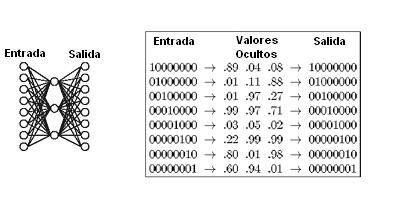
\includegraphics[scale=0.4,bb=0 0 406 203]{red1.png}
  \caption{ Ejemplo esquem�tico de una ANN.}
\end{figure}

\bigskip 
Dicho esto la elecci�n de una red neuronal como medio de resoluci�n del problema de reconocimiento de patrones ser�a en este caso la m�s acertada. Es muy �til cuando no se conoce la funci�n objetivo y se estima que los datos de entrada llegan con cierto porcentaje de ruido. La decisi�n se tom� meses antes de empezar el proyecto. Para asegurarnos de que era viable implementamos la red dentro de un peque�o programa, que a partir de im�genes de entrada devolv�a cierto si detectaba una imagen de una persona con una guante blanco y falso si no hab�a guante.

\section{Descripci�n t�cnica}
Hemos utilizado una red multicapa, ya que permiten representar superficies de decisi�n no lineales. Debido a esto no se puede utilizar unidades lineales ya que solo permitir�an representar funciones lineales. Tampoco pudimos utilizar perceptrones porque su funci�n de salida es discontinua, no derivable y por lo tanto no se le puede aplicar el descenso del gradiente. Necesit�bamos una unidad que diese como salida una funci�n no lineal y que fuese derivable con respecto a las entradas.

\bigskip 
Por eso utilizamos el sigmoide como unidad.

\begin{figure}[h]
  \centering
  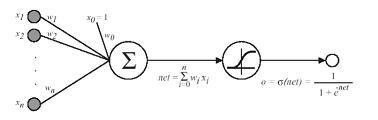
\includegraphics[scale=0.5,bb=0 0 378 120]{red2.png}
  \caption{ Unidad Sigmoide.}
\end{figure}

La funci�n sigma  $ \sigma(x)  = \frac{1}{(1+e^{-x})} $ es no lineal y derivable $ \frac{d\sigma(x)}{dx} =  \sigma(x) . (1 - \sigma(x)) $.

El descenso de gradiente se puede utilizar para entrenar:
\begin{itemize}
\item Una unidad sigmoide.
\item Una red multicapa de unidades sigmoides. Retropropagaci�n.
\end{itemize} 

La retropropagaci�n permite aprender los pesos para una red multicapa con un numero de unidades e interconexiones dado. Consideramos una red con m�ltiples unidades de salida, de forma que el error es la suma de los errores sobre todas las salidas. El espacio de hip�tesis viene dado por los valores posibles para los pesos de todas las unidades de red. Utilizamos el descenso de gradiente para encontrar una hip�tesis que minimice el error, el descenso utilizado es incremental, es decir, los pesos se actualizan despu�s de considerar cada ejemplo de entrenamiento en lugar de esperar a considerarlos todos. Es mas improbable que el descenso incremental caiga en un m�nimo local.
\bigskip 

La secuencia de pasos utilizada en nuestro entrenamiento viene a ser esta:
\begin{itemize}
\item Crear la red. 
\item Se inicializan los pesos de la red con valores peque�os y aleatorios entre -0.05 y 0.05
\item Para una media de 30 iteraciones se realiza lo siguiente: De una lista de im�genes de entrenamiento se va cogiendo una a una y se cargan en la capa de entrada de la red, para esa imagen se calculan las capas, luego seg�n un objetivo se calculo el error cometido en la capa oculta y en la salida y respecto a estos errores se reajustan los pesos de las interconexiones.
\item Se realiza un prueba y una validaci�n con im�genes distintas a las del entrenamiento, para ver el porcentaje de error total cometido, si es aceptable se guarda en un archivo los pesos de la red entrenada, para que en la fase de reconocimiento de im�genes solo haya que realizar el calculo de capas.
\end{itemize} 	

Para cada unidad de salida k, se calcula su termino de error: $ \delta_{k} = O_{k} . (1 - O_{k}) . (t_{k} - O_{k}) $

Para cada unidad oculta h, se calcula su termino de error: $ \delta_{h} = O_{h} . (1 - O_{h}) . \Sigma (W_{kh} . \delta_{k}) $ , siendo k las salidas.

Se actualiza cada peso de la red $ W_{ji} = W_{ji} + \Delta (W_{ji}) $ donde $ \Delta (w_{ji}) = \eta .\delta_{j} .x_{ji} + \alpha .\Delta w_{ji}. (n-1) $. 

($ t_{k} $ es la salida dada por ejemplo de entrenamiento para la unidad k. $ o_{t} $ es la salida generada por la red.)

La actualizaci�n de los pesos en la iteraci�n n depende de la actualizaci�n en n-1. El 2� termino de la ecuaci�n representa la cantidad de movimiento. Un s�mil f�sico seria una pelota que cae por la superficie de error, la cantidad de movimiento hace que la pelota tienda a mantener la misma direcci�n, con esto se intenta evitar que la pelota pare en un m�nimo local o que se pare en un llano.

\bigskip 
Respecto el descenso del gradiente en el sigmoide:
Para el descenso incremental consideramos el cambio en los pesos inducido por cada ejemplo de entrenamiento $ \Delta w_{ji} = \eta \frac{\eta E_{d}}{\eta w_{ji}} $ donde el error sobre un ejemplo de entrenamiento viene dado por la suma de los errores en cada unidad de salida $ E_{d}(w) \equiv \frac{1}{2} . \Sigma (t_{k} - o_{k})^{2} $ , siendo k las salidas

La salida viene dada por $ net = \Sigma w_{i}.x_{i} $ , i=0..n y $ o = \sigma (net) = \frac{1}{1 + e^{-net}} $, aplicando la regla de la cadena $ \frac{\eta E_{d}}{\eta w_{ji}} = \frac{\eta E_{d}}{\eta net_{j}} . \frac{\eta net_{j}}{\eta w_{ji}} = \frac{\eta E_{d}}{\eta net_{j}} . x_{ji} $. Para calcular $ \frac{\eta E_{d}}{\eta net_{j}} $ distinguimos el caso de las unidades de salida y las ocultas.

Error en las unidades de salida $ \frac{\eta E_{d}}{\eta net_{j}} = -(t_{j} - o_{j}). o_{j} .(1 - o_{j}) $. Error en la unidades ocultas $ \frac{\eta E_{d}}{\eta net_{j}} = o_{j} . (1 - o_{j}) . \Sigma (-\delta_{k} . w_{kj})  $.

\bigskip 
Para valores peque�os de los pesos (al principio del proceso) la red presenta una funci�n casi lineal donde es menos probable encontrar m�nimos locales. Cuando la funci�n es mas compleja (un punto mas avanzado del proceso) es de esperar que nos hayamos acercado tanto al m�nimo global que los m�nimo locales sean aceptables. Para garantizar que alcanzamos el m�nimo global utilizamos heur�sticas:
\begin{itemize}
\item A�adiendo cantidad de movimiento.
\item Utilizando descenso incremental.
\item Entrenar distintas redes con los mismos ejemplos, pero con distintos valores iniciales en los pesos.
\end{itemize} 

La capacidad expresiva de este tipo de red es bastante alta ya que:
\begin{itemize}
\item Cualquier funci�n booleana se puede representar con una red de dos capas.
\item Cualquier funci�n continua se puede aproximar con un error arbitrariamente peque�o por una red de dos capas.
\item Cualquier funci�n se puede aproximar con un error arbitrariamente peque�o por una red de tres capas (las dos ocultas de sigmoides y la de salida de unidades lineales).
\end{itemize} 

\section{Dise�o}
Esta formada por una capa de entrada, una de salida y una sola capa oculta.
Si imagin�semos la red como una caja negra, esta tendr�a que recibir como entrada una imagen y sacar como salida una cadena de texto explicativa de alg�n atributo de esa imagen.

\bigskip 
En nuestro caso la entrada ser�n siempre im�genes del mismo tama�o 320x240 p�xeles, por ello la capa de entrada consta de 76800 unidades. En realidad la entrada es un unsigned char* que representa la imagen con valores de 255 o 0, es decir, blanco o negro, recuerdo que las im�genes que le llegan a la red son im�genes que previamente han pasado por el modulo de filtro a si que llegan ya binarizadas. Estas entradas ser�n normalizadas entre 1 y 0, para que las entradas est�n en el mismo rango que las unidades de la capa oculta y de salida.

\bigskip 
La capa oculta debe tener tan pocas unidades como sea posible. Medidas experimentales demuestran que el hecho de aumentar el n�mero de  unidades ocultas proporciona mejoras poco significativas en la precisi�n, pero requieren mucho mas tiempo de entrenamiento. Nosotros hemos optado por utilizar 15 unidades.

\bigskip 
Como ya sabemos al robot se le controla con 2 manos, los gestos de la mano izquierda le indican las ordenes y los de las derecha los par�metros, con el objetivo de simplificar el dise�o los gestos de ordenes y de par�metros son los mismos, pero significan cosas distintas. Tanto para ordenes como para par�metros hay 5 tipos de gestos. Como recordatorio las ordenes eran: parar, avanzar, girar a la izquierda y girar a la derecha. Y los par�metros eran nula, medio baja, medio alta, alta si la orden actual es la de avanzar, donde los par�metros indican la velocidad a la que debe hacerlo o 0�, 45�, 90�, 180� si la orden actual es una de giro. La 5� gesto tanto para ordenes como para par�metros es el ``gesto no reconocido''. Por tanto dado que hay 5 tipos de gestos ha reconocer, la red tendr� que sacar 5 posibles salidas. Al principio optamos por una capa de salida de una sola unidad. El valor oscila entre 0 y 1 as� que por ejemplo si esta unidad val�a 0.2 significaba que hab�a reconocido el 2� gesto, si val�a 0.8 hab�a reconocido el 4� gesto. Luego se cambio al dise�o actual que es una capa de salida de 5 unidades, esto hace a la red mucho mas fiable, se pod�a decir que la salida de la red antes era anal�gica y ahora es digital, ya que todas las salidas tendr�n valores menores de 0.5 excepto una que ser� mayor, solo hay que asociar la unidad de la salida que se ha puesto en alta con una cadena de texto. Esta asociaci�n se hace mediante un script en Lua, as� es m�s modificable ya que si se quiere cambiar el texto de salida no hay que recompilar el proyecto, solo cambiar un archivo de texto.

\bigskip 
La organizaci�n de red por capas es est�ndar, la salida de cada unidad alimenta a todas las unidades de la siguiente capa.

La tasa de aprendizaje utilizada ha sido 0.3. La mas alta posible para reducir el tiempo de aprendizaje sin disminuir la precisi�n.

El descenso de gradiente es incremental para reducir el riesgo de quedarnos en m�nimos locales.

Los pesos de la unidades de salida y oculta son inicializados con peque�os valores aleatorios entre 0.05 y -0.05.

\section{Entrenamiento}
La mayor parte del c�digo utilizado en la red esta dirigido al entrenamiento. Por eso decidimos hacer un programa aparte que contiene el c�digo de entrenamiento de la red y luego el c�digo que est� presente en el proyecto que solo contiene el necesario para crear una red, calcular los valores de las capas a partir del valor de la capa de entrada y generar la cadena de texto de salida. As� el c�digo del proyecto queda mas sencillo para leer.

\bigskip 
El proceso de entrenamiento empieza con la sesi�n fotogr�fica, es necesario hacer mas de un centenar de fotos para obtener un entrenamiento medianamente fiable. Nosotros para el entrenamiento de ordenes sacamos 185 fotos, consiste en sacar fotos d�ndole ordenes al robot correctas, err�neas o simplemente no d�ndoselas. Todas estas fotos han de ser filtradas del mismo modo que lo har�a el modulo de filtro del proyecto, la raz�n de hacer un filtrado previo es poder pasar a la red im�genes muy simples, tambi�n deben de ser tomadas en unas condiciones de iluminaci�n similares a las que tendr� el entorno por el que circule el robot. No es lo mismo hacer aprender a la red a reconocer un gesto perdido en un mar de p�xeles de miles de colores a reconocer un conjunto de p�xeles blancos centrados sobre un fondo negro. Los objetivos mas perseguidos en este proyecto es la eficiencia y en este caso la fiabilidad en el reconocimiento.

\bigskip 
Las fotos son nombradas con un formato determinado, por ejemplo, ``\_orden\_parada\_21.bmp'' esto significa que la foto contiene la orden de parada y ``\_no\_gesto\_51.bmp'' indica que la foto no representa ninguna orden para el robot. Este formato es utilizado en el entrenamiento para que la red sepa ir reajustando los pesos seg�n el nombre explicativo de la foto.

\begin{figure}[h]
  \centering
  \includegraphics[scale=0.5,bb=0 0 160 120]{_no_gesto_36.png}
  \caption{ \_no\_gesto\_36.png}
\end{figure}

Todas las fotos no son utilizadas para el entrenamiento. Se hacen 3 listas de fotos que se utilizaran para el entrenamiento, la prueba y la validaci�n. Estas 2 ultimas sirven  para comprobar el buen funcionamiento de la red entrenada.

El objetivo del programa de entrenamiento es crear una red, entrenarla y salvar la estructura y pesos de red en un archivo.

El entrenamiento consiste en :
\begin{itemize}
\item Recorrer la lista de im�genes de entrenamiento una por una.
\item Cargar la imagen en la imagen en la capa de entrada, cada valor de p�xel se asocia a una unidad de la capa.
\item Seg�n el nombre de la foto, ejemplo ``\_orden\_parada\_21.bmp'', se cambia el objetivo, esto sirve para calcular el error cometido.
\item Cambiado el objetivo, se calcula el valor de la capas respecto a la capa de entrada, se calcula el error cometido en las capas oculta y salida y se reajustan los pesos, para disminuir el error.
\item Esta lista es recorrida un numero finito de iteraciones. Las condiciones de parada pueden ser varias. La nuestra es simplemente un numero concreto, en este caso fueron 30 iteraciones. Por tanto los pesos fueron ajustados 30x(numero de fotos de la lista) veces.
\end{itemize}
Ya tendr�amos as� unos pesos que representan una aproximaci�n a la funci�n buscada.
\bigskip 

\begin{figure}[h]
  \centering
  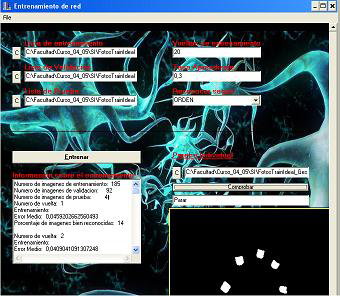
\includegraphics[scale=0.4,bb=0 0 340 296]{prog_train.png}
  \caption{ Captura de nuestro programa de entrenamiento de redes.}
\end{figure}

\bigskip 
Estos fueron datos de un entrenamiento de la red:
\begin{itemize}
\item Datos entrada:
\begin{itemize}
\item 148 fotos de entrenamiento, 49 fotos de validaci�n y 30 de prueba.
\item �ndice de aprendizaje: 0.3
\item 20 iteraciones
\end{itemize} 
\item Datos salida:
\begin{itemize}
\item Porcentaje de aciertos en entrenamiento: 89   Error medio: 0,0141046521582562
\item Porcentaje de aciertos en validaci�n: 93    Error medio: 0,00799933215976971
\item Porcentaje de aciertos en prueba: 100     Error medio: 0,00645778571591585
\end{itemize} 
\end{itemize}   

\begin{figure}[h]
  \centering
  \includegraphics[scale=0.4,bb=0 0 504 231]{Grafica_Aciertos.png}
  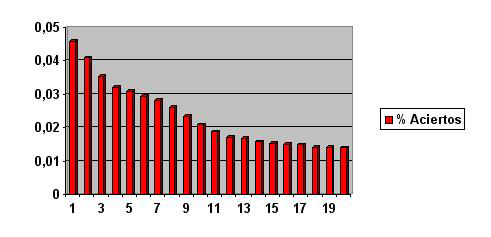
\includegraphics[scale=0.4,bb=0 0 491 237]{Grafica_Errores.png}
  \caption{ La imagen de la izquierda muestra como aumenta el aprendizaje cuanto mas se ense�a a la red. Aumentando el n� de aciertos. Y la de la derecha muestra como a medida que aprende comete menos errores reconociendo figuras.}
\end{figure}

\section{Red Neuronal en el proyecto}
Como cada modulo del pipeline, el modulo de red tiene un peque�o numero de funciones fijas utilizadas para ser llamadas desde el pipeline. Tres de ellas son ``red\_iniciar'', ``red\_cerrar'' y ``red\_ciclo''. Iniciar crea la red y carga el archivo creado por el programa de entrenamiento, por ejemplo el ``orden\_net''. La funci�n cerrar libera toda la memoria. Y la funci�n ciclo lo �nico que hace es recibir un char* que representa la imagen, cargar estos valores normalizados en la capa de entrada y calcular el valor de las capas oculta y de salida seg�n los pesos, que solamente tarda aproximadamente 0.10 segundos. Luego como ya dijimos solamente una de las cinco unidades de la capa de salida tendr� un valor superior a 0.5, esto es equivalente a que se ha puesto en ALTA y el modulo sacar� como salida la cadena de texto asociada a esa unidad. Cadena modificable desde un script junto con el nombre del archivo de la red entrenada. Todo lo que sea modificable en un futuro por posibles mejoras son par�metros que van escritos en scripts.

\bigskip 
Estas son 5 im�genes filtradas de ejemplo, cada una representa una orden o un par�metro.

Recordatorio:
\begin{itemize}
\item 1 dedo: Orden: Avanzar, Par�metro:  Medio baja o 45�
\item 2 dedos: Orden: Girar derecha,  Par�metro:  Medio alta o 90�
\item 3 dedos: Orden: Girar Izquierda,  Par�metro:  Alta o 180�
\item  5 dedos: Orden: Parar ,  Par�metro:  Nula o 0�
\end{itemize} 
 
\begin{figure}[h]
  \centering
  \includegraphics[scale=0.4,bb=0 0 160 120]{_orden_parada_17.png}
  
\includegraphics[scale=0.4,bb=0 0 160 120]{_orden_avanza_38.png}
  
\includegraphics[scale=0.4,bb=0 0 160 120]{_orden_angulo_43.png}
  \includegraphics[scale=0.4,bb=0 0 160 120]{_orden_negAngulo_84.png}
  \caption{ Ejemplos de imagenes de entrada en la red.}
\end{figure}

\section{Evoluci�n}
El primer sistema utilizado para resolver el problema de reconocimiento de gestos, fue la implementaci�n de dos redes distintas una para ordenes y otra para par�metros, debido a que su estructura era distinta.

Se fueron modificando los filtros con el objetivo de facilitar el aprendizaje a la red.

La segunda elecci�n fue utilizar el mismo numero de gestos tanto en ordenes como en par�metros as� se pudo conseguir la misma implementaci�n para ambas.

Luego se redujo considerablemente el c�digo, eliminando la parte de entrenamiento del proyecto. El c�digo de entrenamiento pasar�a a ser un programa a parte que generar� archivos de redes entrenadas. En este punto hab�a 2 archivos uno para cada red.

Y por ultimo visto que los gestos de las ordenes eran reconocidos con mucha mas facilidad que los asignados a los par�metros, que fallaban constantemente, decidimos que los gestos de los par�metros fuesen iguales a los de las ordenes, solo que en vez de hacer gestos con la izquierda se hacen con la derecha. De esta manera ambas redes cargan el mismo archivo y son igual de fiables. Solo se diferencian por la cadena de texto que devuelven, pero eso va por scripts.

\section{C�digo}
Ver anexo: documentaci�n del m�dulo de red.c y red\_neuronal.c, en \ref {red_code} (p�gina \pageref{red_code}).


\chapter{M�dulo de gesti�n de mensajes}

\section{Introducci�n}
Este m�dulo de la aplicaci�n tiene como misi�n recoger todos los mensajes que han podido ser generados por m�dulos de proceso anteriores, y filtrarlos de tal modo que la salida de la l�nea de ejecuci�n est� dotada de cierta coherencia con el resultado deseado. Para ello, admite las entradas en forma de cadenas de texto, y elige cu�les de ellas son las que deber�an dar realmente una salida a los m�dulos posteriores.

\section{Detalles}
\begin{itemize}
  \item {\bf Entrada}: Cualquier cadena de texto, y par�metros para controlar la tolerancia.
  \item {\bf Salida}: Una cadena de texto, la que m�s se asemeja a la que realmente deber�a ser generada.
  \item {\bf Descripci�n}: M�dulo que, a trav�s de la parametrizaci�n, guarda una tabla con las entradas, y, en funci�n de las cantidades de informaci�n, presenta la mejor salida.
\end{itemize}

\section {Arquitectura y funcionamiento del m�dulo}

El m�dulo trabaja con una \emph{tabla hash} inicialmente vac�a. Cuando recibe se�ales procedentes del m�dulo procesador, realiza una de las dos opciones siguientes:

\begin{enumerate}
\item \textbf{El elemento no estaba en la tabla}: Se a�ade a la tabla y se suma una unidad.
\item \textbf{El elemento ya estaba en la tabla}: Se suma una unidad al n�mero de llegadas consecutivas de ese elemento.
\end{enumerate}
Tras este primer paso, se procede a la ``debilitaci�n'' de las otras se�ales. Con esto queremos decir que reducimos el �ndice de refuerzo asociado a todas las se�ales que no fueran la que hemos escogido para que impere, tras una serie de ciclos que parametrizamos a trav�s de los argumentos del m�dulo, la se�al m�s importante (la que m�s veces seguidas ha llegado), que consideramos como la real que deber�a ser transmitida.

De esta forma, siempre mantenemos en la tabla todas las se�ales que van llegando, y creamos un tipo de diagrama de estados borroso, en el que el estado principal es decidido mediante los valores que el m�dulo va asignando a cada registro de la tabla.

Como utilidad a�adida, este m�dulo es uno de los m�s gen�ricos del \emph{pipeline}. El hecho de que los estados posibles se vayan creando de forma din�mica, y que sean s�lo diferenciados por una cadena de texto, ha hecho posible que el m�dulo sea usado para gestionar diferentes l�neas, sin tener que modificar ni una l�nea de c�digo. La �nica parte que hay que personalizar son los par�metros de la instanciaci�n del m�dulo, para que el comportamiento sea lo mejor posible.

?\chapter{M�dulo de control del robot}

\section{Introducci�n}
El m�dulo de control de robot ha sido creado con el fin de tener una pieza de software capaz de controlar nuestro robot de una forma sencilla y transparente para los m�dulos que generan la informaci�n de salida. A este m�dulo le llega una estructura de datos que contiene la orden y el par�metro, y el robot se encarga de moverse en funci�n de esa informaci�n. A continuaci�n detallamos c�mo lo hace.

\section{Arquitectura del m�dulo}
El m�dulo en s� tiene una estructura muy simple: consiste en un conjunto de funciones que son exportadas a un \emph{script} programado en el lenguaje \textbf{Lua}, y que funcionan principalmente haciendo llamadas a una librer�a que hemos creado, y que se encarga de controlar el puerto paralelo.

\subsection{Scripts}
La verdadera programaci�n de la funci�n del robot la hemos delegado en un \emph{script}. Este m�todo de programaci�n nos permite m�s flexibilidad a la hora de controlar el comportamiento de la m�quina.

En el script del robot implementamos algunas funciones determinadas que necesita el m�dulo de control, y las que nosotros deseemos. En este c�digo definimos de una manera muy simple qu� tiene que hacer el robot (realmente el puerto paralelo) cuando le llegan las �rdenes de los otros m�dulos.

\subsection{Biblioteca de control del puerto paralelo}
Hemos desarrollado una biblioteca que provee un interfaz lo m�s simple posible de control de los pines del puerto paralelo, y que adem�s es \textbf{multiplataforma}. A trav�s de ella se puede controlar los pines del cable, con llamadas simples, en las cuales s�lo hay que especificar que pin se quiere usar, y si se quiere poner a \emph{alta} o a \emph{baja}. De este modo nos hemos abstra�do, en la implementaci�n del m�dulo en s�, de las peque�as dificultades que puede ocasionar interactuar directamente con la entrada/salida del ordenador.

Para la implementaci�n de esta biblioteca hemos usado a su vez dos bibliotecas externas: \textbf{parapin} para la implementaci�n en GNU/Linux, y la DLL \textbf{inpout32.dll} para el uso en plataformas Win32.

\section{Construcci�n del robot}
Para construir la estructura f�sica del robot, hemos usado piezas de \emph{Lego Technics}. Este material es barato y razonablemente consistente para soportar su propio peso, el de la c�mara, el circuito, y el cable paralelo. Adem�s, destaca principalemente por su versatilidad de uso y su capacidad de reconstrucci�n. El ensamblado de las piezas es inmediato (hay que tener en cuenta que se vende como juguete para ni�os a partir de 12 a�os), y los errores de estructura se pueden subsanar con mucha facilidad.

Sin embargo, hemos escogido este material por la facilidad que hemos encontrado para generar m�quinas m�viles. Los conjuntos de piezas de \emph{Lego Technics} suelen venir acompa�ados por estructuras m�s complejas de construcci�n, como motores y brazos hidr�ulicos, elementos que hemos usado para nuestro robot.

El circuito ha sido conectado sobre una placa peque�a de entrenador, a pesar de su fiabilidad relativa, es r�pida de montar y de depurar. Hemos usado un chip \textbf{L293B}, que sirve para control de motores bidireccionales de corriente cont�nua, y alimentamos el circuito con una pila de 9 voltios. El circuito que usa el robot es el de la figura \ref{circuito_robot}.

%\usepackage{graphics} is needed for \includegraphics
%\begin{figure}[htp]
\begin{figure}[h]
\begin{center}
  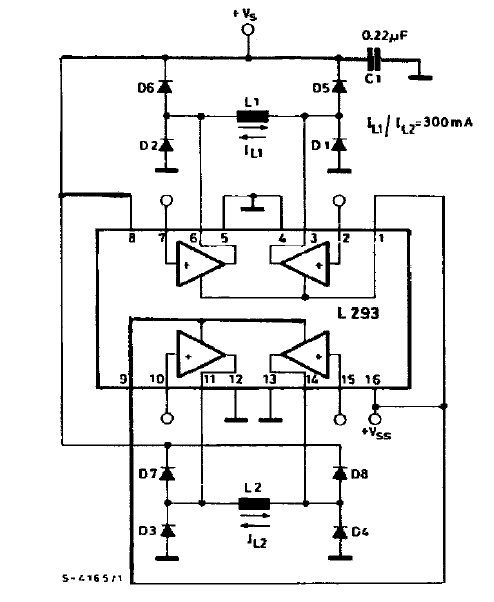
\includegraphics[scale=0.5,bb=0 0 494 602]{circuito.png}
  \caption{Cirtuito de control robot con chip \emph{L293B}}
  \label{circuito_robot}
\end{center}
\end{figure}

\section {Fotos}
A continuaci�n mostramos algunas fotos del robot que hemos construido:
% TODO: pues tud�

\begin{figure}[h]
  \centering
  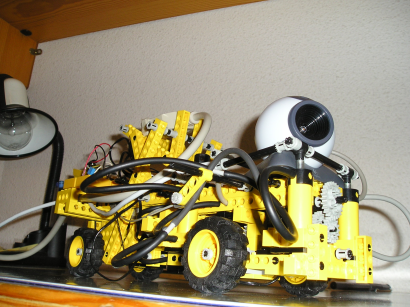
\includegraphics[scale=0.5,bb=0 0 410 307]{robot6.png}
% robot1.png: 72.009dpi, width=5.68cm, height=4.27cm, bb=0 0 161 121
  \caption{Foto lateral del robot}
\end{figure}

\begin{figure}[h]
  \centering
  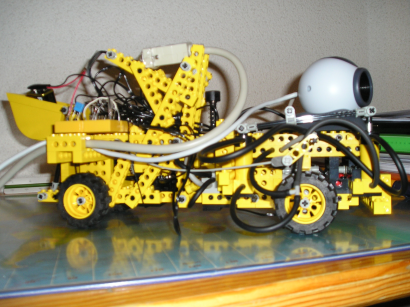
\includegraphics[scale=0.5,bb=0 0 410 307]{robot1.png}
% robot1.png: 72.009dpi, width=5.68cm, height=4.27cm, bb=0 0 161 121
  \caption{Foto inferior del robot}
\end{figure}





\section {C�digo}
% TODO: poner bien la referencia
Ver anexo: documentaci�n del m�dulo de robot.c, en \ref {robot_8c} (p�gina \pageref{robot_8c}).
\chapter{Procesamiento de texto reconocido}

\section{Introducci�n}
Una vez que el OCR ha reconocido una cadena de texto y la ha validado, env�a la se�al a este m�dulo, que se encarga de procesarlo, y crear una nueva salida en el formato propio del pipeline para el entorno 3D y el robot.

\section{Implementaci�n}

Para implementarlo, hemos usado un programa en \textbf{Prolog}, que est� formado en su mayor parte por una DCG \footnote{Definite clause grammar}. Este programa recibe la entrada del m�dulo, y, tras procesarla, crea una salida, que puede ser una cadena de respuesta, el resultado de una operaci�n aritm�tica (soporta par�ntesis y anidamiento de expresiones) o una orden para la salida.

\section{Ampliabilidad}

La idea de crear el m�dulo como antes hemos explicado ha sido propiciada por la idea de que la ``inteligencia del robot'' fuese algo ampliable. Con s�lo modificar este archivo, se puede dotar a la m�quina de m�s informaci�n (ampliando el diccionario), o de m�s capacidad de proceso (creando m�s reglas de reconocimiento en la DCG).

\section {C�digo}
% TODO: poner bien la referencia
Ver anexo: documentaci�n del m�dulo de prolog.c, en \ref {prolog_8c} (p�gina \pageref{prolog_8c}).
\chapter {Otros m�dulos}

\section{Introducci�n}
A continuaci�n explicamos el funcionamiento del resto de los m�dulos. Los aglutinamos en esta secci�n, por carecer de inter�s la explicaci�n detallada de los mismos, debido a su sencillez.

% TODO: poner las referencias

\section {M�dulo de post-gesti�n}
Hemos a�adido un m�dulo que recoja todas las se�ales que son generadas por las distintas ramas de proceso del \emph{pipeline}, y las agrupe en una sola salida v�lida, para ofrecer de este modo, a trav�s de sus puertos, datos a todos los m�dulos de salida.

Adem�s, hemos incluido en el m�dulo la posibilidad de generar salidas en un script, para que la depuraci�n de los m�dulos no dependa de los que est�n m�s arriba en el grafo, y tener m�s potencia de control de errores.

Puede examinar su documentaci�n de c�digo en \ref{caca}.

\section{Ventana de par�metros}
La ventana de par�metros es una interfaz gr�fica en la que es posible elegir un color, y tres tolerancias (una para el rojo, otra para el verde y otra para el azul), y alimentar as� a un m�dulo de filtro, de tal modo que la parametrizaci�n de los valores del mismo se pueda hacer en tiempo real.

Puede examinar su documentaci�n de c�digo en \ref{caca}.

\section{Ventana de im�genes}
La ventana de im�genes es simplemente un m�dulo que muestra gr�ficamente, en una ventana que se redimensiona autom�ticamente, una imagen que sigue el formato propio de nuestra aplicaci�n (ver secci�n \ref{formato_imagenes}).

La ventana de im�genes tiene como funci�n a�adida la capacidad de guardar una toma de la imagen que se este dibujando en el instante en el que se pulsa \textbf{F5}.

Puede examinar su documentaci�n de c�digo en \ref{caca}.

\section{M�dulo de control de joystick}
Hemos a�adido tambi�n al pipeline un m�dulo que, a trav�s de un interfaz de joystick, puede traducir sus entradas a las correspondientes �rdenes y par�metros del robot y del entorno 3D. De esta forma, la depuraci�n es sencilla y r�pida.

Para la implementaci�n hemos utilizado las bibliotecas SDL (Simple Directmedia Library).

Puede examinar su documentaci�n de c�digo en \ref{caca}.

\section{M�dulo de salida}
Este m�dulo es simplemente una ventana con un cuadro de texto que es capaz de imprimir en �l todas las cadenas (en formato C, \verb|char *|) que le llegan a trav�s de sus puertos.

Puede examinar su documentaci�n de c�digo en \ref{caca}.
% \chapter{Introduccion a redes neuronales}
\label{Introduccion_redes} 

Las Redes Neuronales Artificiales (ANNs de Artificial Neural Networks) fueron originalmente una simulaci�n abstracta de los sistemas nerviosos biol�gicos, formados por un conjunto de unidades llamadas "neuronas" o "nodos" conectadas unas con otras. Estas conexiones tienen una gran semejanza con las dendritas y los axones en los sistemas nerviosos biol�gicos. 

El Primer modelo de red neuronal fue propuesto en 1943 por McCulloch y Pitts en t�rminos de un modelo computacional de "actividad nerviosa". El modelo de McCulloch-Pitts es un modelo binario, y cada neurona tiene un escal�n o umbral prefijado. Este primer modelo sirvi� de ejemplo para los modelos posteriores de Jhon Von Neumann, Marvin Minsky, Frank Rosenblatt, y muchos otros. 

Pongamos de ejemplo el cerebro humano:
\begin{itemize}
\item Formado por una red de neuronas interconectadas.
\item $ 10^{10} $ neuronas en el cerebro humano.
\item Tiempo de conmutaci�n 0,001 segundo (computadora: $ 10^{-10} $).
\item Tiempo que se tarda en reconocer una imagen: 0.1 segundo.
\item 100 pasos de procesamiento parecen pocos para resolver un problema tan complejo como el reconocimiento de im�genes.
\item Hip�tesis: el cerebro humano presenta un paralelismo masivo sobre una representaci�n distribuida.
\end{itemize} 	

Debido a la inspiraci�n ya mencionada de las ANN en el cerebro, sus aplicaciones principales estar�n centradas en campos donde la inteligencia humana no pueda ser emulada de forma satisfactoria por algoritmos aritm�ticos que pueden ser implementados en ordenadores. Adem�s es de prever que dichas ANN tengan caracter�sticas similares a las del cerebro: 
\begin{itemize}
\item Ser�n robustas i tolerantes a fallos. En el cerebro mueren todos los d�as gran cantidad de neuronas sin afectar sensiblemente a su funcionamiento.
\item Ser�n flexibles. El cerebro se adapta a nuevas circunstancias mediante el aprendizaje .
\item Podr�n trabajar con informaci�n borrosa, incompleta, probabil�stica, con ruido o inconsistente. 
\item Ser�n altamente paralelas. El cerebro esta formado por muchas neuronas interconectadas entre si y es precisamente el comportamiento colectivo de todas ellas lo que caracteriza su forma de procesar la informaci�n.
\end{itemize} 
Resumiendo una ANN es un gran numero de conmutadores interconectados, donde a las conexiones se les asigna un peso. Este peso ser� fijado durante la fase de aprendizaje. El procesamiento de informaci�n es paralelo distribuido.

En que tipos de problemas se utilizan:
\begin{itemize}
\item En problemas donde los ejemplos se describen con un gran numero de atributos.
\item Puede haber ruido en los datos.
\item Cuando no se conoce la forma de la funci�n objetivo. Problemas que no tienen un algoritmo especifico para su soluci�n, o cuyo algoritmo es demasiado complejo para ser encontrado. 
\item Cuando es permisible un tiempo de entrenamiento largo.
\item Ejemplos: Reconocimiento del habla, clasificaci�n de im�genes, predicciones financieras, etc.
\end{itemize} 

\begin{figure}
  \centering
  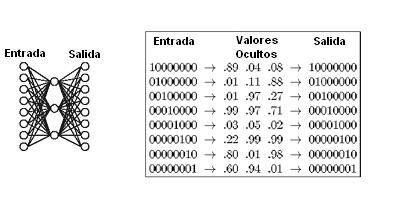
\includegraphics[scale=0.5,bb=0 0 406 203]{red1.png}
  \caption{ red1.png}
\end{figure}

Existen dos fases en toda aplicaci�n de las redes neuronales: la fase de aprendizaje o entrenamiento y la fase de prueba. En la fase de entrenamiento, se usa un conjunto de datos o patrones de entrenamiento para determinar los pesos (par�metros de dise�o) que definen el modelo neuronal. Una vez entrenado este modelo, se usar� en la llamada fase de prueba o funcionamiento directo, en la que se procesan los patrones de prueba que constituyen la entrada habitual de la red, analiz�ndose de esta manera las prestaciones definitivas de la red.

En general, las Redes Neuronales Artificiales han sido claramente aceptadas como nuevos sistemas muy eficaces para el tratamiento de la informaci�n en muchas disciplinas. Ellos ha dado como resultado una variedad de aplicaciones comerciales (tanto en productos como en servicios) de esta tecnolog�a de redes neuronales.


% \chapter{Descripci�n T�cnica}

\hline

Hemos utilizado una red multicapa, ya que permiten representar superficies de decisi�n no lineales. Debido a esto no se puede utilizar unidades lineales ya que solo permitir�an representar funciones lineales. Tampoco pudimos utilizar perceptrones porque su funci�n de salida es discontinua, no derivable y por lo tanto no se le puede aplicar el descenso del gradiente. Necesit�bamos una unidad que diese como salida una funci�n no lineal y que fuese derivable con respecto a las entradas.
Por eso utilizamos el sigmoide como unidad.

\begin{center}
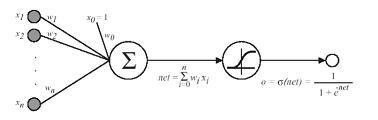
\includegraphics[scale=1]{red2.png} 
\end{center} 

La funci�n sigma $ \sigma(x) = \dfrac{1}{1 + e^{-x}} $   es no lineal y derivable $ \dfrac{d\sigma(x)}{dx} = \sigma(x) . (1 - \sigma(x)) $.
El descenso de gradiente se puede utilizar para entrenar:
\begin{itemize}
\item Una unidad sigmoide.
\item Una red multicapa de unidades sigmoides. Retropropagaci�n.
\end{itemize} 

La retropropagaci�n permite aprender los pesos para una red multicapa con un numero de unidades e interconexiones dado. Consideramos una red con m�ltiples unidades de salida, de forma que el error es la suma de los errores sobre todas las salidas. El espacio de hip�tesis viene dado por los valores posibles para los pesos de todas las unidades de red. Utilizamos el descenso de gradiente para encontrar una hip�tesis que minimice el error, el descenso utilizado es incremental, es decir, los pesos se actualizan despu�s de considerar cada ejemplo de entrenamiento en lugar de esperar a considerarlos todos. Es mas improbable que el descenso incremental caiga en un m�nimo local.

La secuencia de pasos utilizada en nuestro entrenamiento viene a ser esta:
\begin{itemize}
\item Crear la red. 
\item Se inicializan los pesos de la red con valores peque�os y aleatorios entre -0.05 y 0.05
\item Para una media de 30 iteraciones se realiza lo siguiente: De una lista de im�genes de entrenamiento se va cogiendo una a una y se cargan en la capa de entrada de la red, para esa imagen se calculan las capas, luego seg�n un objetivo se calculo el error cometido en la capa oculta y en la salida y respecto a estos errores se reajustan los pesos de las interconexiones.
\item Se realiza un prueba y una validaci�n con im�genes distintas a las del entrenamiento, para ver el porcentaje de error total cometido, si es aceptable se guarda en un archivo los pesos de la red entrenada, para que en la fase de reconocimiento de im�genes solo haya que realizar el calculo de capas.
\end{itemize} 	

Para cada unidad de salida k, se calcula su termino de error: $ \delta_{k} = O_{k} . (1 - O_{k}) . (t_{k} - O_{k}) $
Para cada unidad oculta h, se calcula su termino de error: $ \delta_{h} = O_{h} . (1 - O_{h}) . \Sigma (W_{kh} . \delta_{k}) $ , siendo k las salidas.
Se actualiza cada peso de la red $ W_{ji} = W_{ji} + \Delta (W_{ji}) $ donde $ \Delta (w_{ji}) = \eta .\delta_{j} .x_{ji} + \alpha .\Delta w_{ji}. (n-1) $. 
(t_{k} es la salida dada por ejemplo de entrenamiento para la unidad k. o_{t} es la salida generada por la red.)
La actualizaci�n de los pesos en la iteraci�n n depende de la actualizaci�n en n-1. El 2� termino de la ecuaci�n representa la cantidad de movimiento. Un s�mil f�sico seria una pelota que cae por la superficie de error, la cantidad de movimiento hace que la pelota tienda a mantener la misma direcci�n, con esto se intenta evitar que la pelota pare en un m�nimo local o que se pare en un llano.

Respecto el descenso del gradiente en el sigmoide:
Para el descenso incremental consideramos el cambio en los pesos inducido por cada ejemplo de entrenamiento $ \Delta w_{ji} = -\eta . \dfrac{\eth E_{d}}{\eth w_{ji}} $
donde el error sobre un ejemplo de entrenamiento viene dado por la suma de los errores en cada unidad de salida $ E_{d}(w) \equiv \frac{1}{2} . \Sigma (t_{k} - o_{k})^{2} $ , siendo k las salidas
La salida viene dada por $ net = \Sigma w_{i}.x_{i} $ , i=0..n y $ o = \sigma (net) = \dfrac{1}{1 + e^{-net}} $, aplicando la regla de la cadena $ \dfrac{\eth E_{d}}{\eth w_{ji}} = \dfrac{\eth E_{d}}{\eth net_{j}} . \dfrac{\eth net_{j}}{\eth w_{ji}} = \dfrac{\eth E_{d}}{\eth net_{j}} . x_{ji} $. Para calcular $ \dfrac{\eth E_{d}}{\eth net_{j}} $ distinguimos el caso de las unidades de salida y las ocultas.
Error en las unidades de salida $ \dfrac{\eth E_{d}}{\eth net_{j}} = -(t_{j} - o_{j}). o_{j} .(1 - o_{j}) $. Error en la unidades ocultas $ \dfrac{\eth E_{d}}{\eth net_{j}} = o_{j} . (1 - o_{j}) . \Sigma (-\delta_{k} . w_{kj})  $.

Para valores peque�os de los pesos (al principio del proceso) la red presenta una funci�n casi lineal donde es menos probable encontrar m�nimos locales. Cuando la funci�n es mas compleja (un punto mas avanzado del proceso) es de esperar que nos hayamos acercado tanto al m�nimo global que los m�nimo locales sean aceptables. Para garantizar que alcanzamos el m�nimo global utilizamos heur�sticas:
\begin{itemize}
\item A�adiendo cantidad de movimiento.
\item Utilizando descenso incremental.
\item Entrenar distintas redes con los mismos ejemplos, pero con distintos valores iniciales en los pesos.
\end{itemize} 

La capacidad expresiva de este tipo de red es bastante alta ya que:
\begin{itemize}
\item Cualquier funci�n booleana se puede representar con una red de dos capas.
\item Cualquier funci�n continua se puede aproximar con un error arbitrariamente peque�o por una red de dos capas.
\item Cualquier funci�n se puede aproximar con un error arbitrariamente peque�o por una red de tres capas (las dos ocultas de sigmoides y la de salida de unidades lineales).
\end{itemize} 

Respecto al sesgo inductivo:
El espacio de hip�tesis es continuo a diferencia de los espacios de hip�tesis de otros m�todos inductivos
Las redes neuronales realizan una interpolaci�n. Dados dos ejemplos positivos que no tienen ejemplos negativos entre ellos se tienden a etiquetar como positivos todos los puntos intermedios


% \section{Filtro de Gestos}
\label{filtro_gestos} 

\subsection{Introducci�n}
Como ya hemos dicho este filtro sirve como preprocesamiento y segmentaci�n de la imagen. Ya que el suavizado reduce los ruidos y la extracci�n de regiones de color localiza los objetos de inter�s, con el objetivo de pasarle una informaci�n mucho mas comprensible y simplificada a la red neuronal.
\bigskip 
Los gestos al robot se realizan con la ayuda de 2 guantes, uno para la mano izquierda que dar� las ordenes y otro para la derecha que indicar� los par�metros para dichas ordenes.

Cada guante tiene en la punta de los dedos unos marcadores de color especial, un color que no se encuentre formando parte del entorno (colores muy llamativos con una textura que no gener� brillos o sombras). 
\bigskip 
Se determinaron una conjunto de ordenes, las justas para que un objeto pueda describir cualquier trayectoria sobre una superficie plana. Concluimos que estas podr�an ser �nicamente: avanzar y girar. Es necesario decirle la distancia que tiene que avanzar en cada momento, pero como eso no era simple, se introdujo la orden parar, as� mientras se mueve el robot tu decides cuando ha recorrido la distancia oportuna y detenerlo con una orden. Tambi�n se distingui� en la orden girar, entre girar a la izquierda y girar a la derecha. Con esto tenemos 4 tipos de ordenes distintas para dar al robot. Pero aun el robot necesita mas informaci�n sobre estas ordenes, como por ejemplo en la orden de giro, con cuantos grados tiene que realizarlo o en la orden de avanzar a cuanta velocidad debe moverse. Siguiendo con el objetivo de la simplicidad en vez de a�adir mas gestos diferentes a la misma mano, se utilizo la otra mano, es decir, una mano indicar�a las ordenes al robot y otra los par�metros seg�n el tipo de orden. 

Los par�metros son o de velocidad o de grados de giro, la velocidad puede ser nula, medio baja, medio alta o alta y los �ngulos de giro pueden ser 0�, 45�, 90� o 180�, es decir, cuatro par�metros en ambos casos, se utilizan los mismos s�mbolos para velocidad como para giro, por tanto solo existen 4 gestos diferentes que se puedan dar con la mano derecha para expresar los par�metros al robot. 

La coincidencia del numero de gestos utilizados para ordenes y el numero de gestos utilizados para par�metros, simplificara la implementaci�n de la red. Y el hecho de usar los mismos gestos para representar las ordenes con la mano izquierda y los par�metros con la mano derecha, simplificara tambi�n el entrenamiento de la red.
\bigskip 
Resumiendo:
\begin{itemize}
\item Mano Izquierda = Ordenes
  \begin{enumerate}
  \item Parar
  \item Avanzar
  \item Girar Izquierda
  \item Girar Derecha
  \end{enumerate} 
\item Mano Derecha = Par�metros
  \begin{enumerate}
  \item Si orden == Avanzar entonces
    \begin{itemize}
    \item Parar
    \item Medio baja
    \item Medio alta
    \item Alta
    \end{itemize} 
  \item Si (orden == Girar Izquierda) or (orden == Girar Derecha) entonces
    \begin{itemize}
    \item 0 �
    \item 45�
    \item 90�
    \item 180�
    \end{itemize} 
  \end{enumerate} 
\end{itemize} 					

Los gestos elegidos son diferentes posiciones de los marcadores del guante, lo mas claro posible, para que despu�s del filtrado la red no tenga problema para diferenciar unos s�mbolos de otros.

Los marcadores son las �nicas �reas de la imagen que no se eliminaran de la imagen. Estas regiones pasar�n a ser blancas y el resto negro. Por tanto repito los gestos tienen que ser los suficientemente distintos unos de otros, para que una vez filtrados, esas zonas blancas puedan diferenciarse a simple vista y saber a que orden se est�n refiriendo. 

Es en ejecuci�n cuando se decide a trav�s de una ventana proporcionada por el pipeline el color de la imagen a filtrar, as� que el color de los marcadores del guante no tienen porque ser fijos, se pueden determinar en cada momento. Eso si, los colores de ambos guantes deben de ser distintos y especificarse que color ser� el que representa a las ordenes y cual representara a los par�metros.
\bigskip 
Estos son los 4 posibles gestos:
\begin{center}
%\includegraphics[scale=1]{parar.png} 
Parada
%\includegraphics[scale=1]{avanzar.png} 
Avanzar
%\includegraphics[scale=1]{girarDcha.png} 
Girar Derecha
%\includegraphics[scale=1]{girarIzq.png} 
Girar Izquierda
\end{center} 

Este ser�a el resultado de aplicar el modulo de filtro de gestos sobre esta imagen con una guante:
\begin{center}
%\includegraphics[scale=1]{parar.png} 
%\includegraphics[scale=1]{filtrado.png} 
\end{center} 

y esta sobre una imagen sin guante:
\begin{center}
%\includegraphics[scale=1]{no_gesto.png} 
%\includegraphics[scale=1]{filtrado_no_gesto.png} 
\end{center} 

Los filtros aplicados para esta simplificaci�n son:
\begin{itemize}
\item Suavizado. Por promediado del entorno.
\item Extracci�n de regiones por el color.
\item Centrado de imagen. 
\end{itemize} 

\subsection{Suavizado de la imagen}
Difumina la imagen. Cuando no se aplica, la extracci�n de regiones posterior no es muy fiable, ya que a causa de la iluminaci�n o de la textura del material utilizado en el color especial, hay zonas del objeto de inter�s que no tienen el mismo color pudiendo pasar por ejemplo de ser un rojo casi blanco a un rojo casi negro, esta amplitud de color es inadmisible para la extracci�n de colores, ya que esos p�xeles ser�an considerados fuera de rango y por tanto como elementos del entorno y no como elementos de inter�s. Esto repercutir�a en la red neuronal posterior, la cual tiene que asignar pesos seg�n el valor de los p�xeles de entrada, si no podemos determinar unos valores fiables en las im�genes de entrada no se podr� entrenar de forma fiable la red ni poder asegurar un comportamiento seguro en el futuro.

El suavizado es una transformaci�n de vecindad, donde el valor del nuevo p�xel depende de los valores de los p�xeles que le rodean. Nuestro m�todo de filtro es un suavizado por el promediado del entorno de vecindad.
\bigskip 

Para saber m�s sobre este filtro: \ref {suavizado_label} (p�gina \pageref{suavizado_label}).

\bigskip 
Gracias a esto, los p�xeles dentro de la regi�n de color de inter�s que sean ruidos generados por reflejos de luz o fallos de iluminaci�n, quedaran mas atenuados y todos los p�xeles dentro de la regi�n tendr�n mas posibilidades de estar dentro del rango de color especial buscado.
\begin{center}
%\includegraphics[scale=1]{suavizado.png} 
\end{center} 

\subsection{Extracci�n de regiones de color}
Como hemos dicho los objetos de inter�s son las puntas de los dedos, as� que tenemos que aislarlas del resto de la fotograf�a. La forma es delimitar estas regiones y darlas toda la importancia respecto al resto de la imagen.

Queremos que el filtro convierta una imagen capturada por la webcam en una imagen blanca y negra, donde las puntas de los guantes quedaran en blanco y el resto de la imagen en negro. As� la red solamente ser� entrenada para recibir im�genes con regiones blancas y negras, si hay una sola regi�n de un cierto tama�o implicar�a que solo hemos ense�ado un dedo del guante, lo que se corresponder�a con el gesto de avanzar. 

Esto es a lo que llamamos segmentaci�n, ya que estamos localizando los objetos de inter�s.
\bigskip 

Para saber mas sobre la extracci�n:  \ref {regiones_label} (p�gina \pageref{regiones_label}).

\begin{center}
%\includegraphics[scale=1]{regiones.png} 
\end{center}  

\subsection{Centrado de la imagen}
Los gestos realizados con los guantes nunca son capturados por la webcam en la misma posici�n. Nunca estar�n totalmente centrados, si no ligeramente o totalmente desplazados mas a la derecho o mas a la izquierda, arriba o abajo. Esto es de vital importancia para la red, ya que entrena y reconoce en relaci�n a los valores de los p�xeles de la imagen, si aprende que el s�mbolo de avanzar es una regi�n blanca sobre un fondo negro situada siempre en el centro de la imagen, cuando este en fase de reconocimiento y la webcam capture un gesto desplazado, la red lo considerara como gesto no reconocido.
Otra opci�n podr�a ser entrenar la red para que reconociese el mismo gesto en cualquier posici�n, pero eso no podr�a nunca servir en el entrenamiento, y que los pesos no terminar�an nunca de fijarse, ya que el p�xel (x,y) si esta blanco para unas im�genes se considerara como ejemplo de entrenamiento positivo, para otras se considerara negativo y los pesos no podr�n ajustarse. Por tanto hay que intentar conseguir que las regiones de inter�s extra�das est�n siempre situadas mas o menos en la misma zona de la imagen. Para eso decidimos que la mejor forma de hacer esto era centrar la imagen seg�n el centro de masas del conjunto de p�xeles de inter�s.

As� siempre las regiones blancas que representan los gestos aparecen centrados en la imagen sobre un fondo negros, totalmente preparados para ser pasados a la entrada de la red neuronal.
\bigskip 

Para saber mas sobre el centrado: \ref {centrado_label} (p�gina \pageref{centrado_label}).

\bigskip 
\begin{center}
%\includegraphics[scale=1]{filtrado.png} 
\end{center} 

\subsection{C�digo}
Documentaci�n del c�digo del filtro de gestos, en \ref {Codigo_filtro_gestos} (p�gina \pageref{Codigo_filtro_gestos}).


% \chapter{Filtros}

La visi�n artificial es el proceso sensorial m�s complejo de todos.
Las tareas en vis�n por computador se pueden enumerar en:
\begin{enumerate}
\item Visi�n de bajo nivel. (Tareas autom�ticas)
  \begin{itemize}
  \item Captaci�n. Obtenci�n de la imagen.
  \item Preprocesamiento. Incluye t�cnicas como reducci�n de ruido y realce de detalles.
  \end{itemize} 
\item Visi�n de nivel medio. (Etiquetar objetos)
  \begin{itemize}
  \item  Segmentaci�n. Localizaci�n de los objetos de inter�s.
  \item Descripci�n. Obtenci�n de caracter�sticas: tama�o, formas, etc.
  \end{itemize} 
\item Visi�n de alto nivel. (Emular inteligencia)
  \begin{itemize}
  \item Reconocimiento. Identificaci�n de objetos: tornillos, puertas, etc.
  \item Interpretaci�n. Significado de un conjunto de objetos.
  \end{itemize} 
\end{enumerate} 

El objetivo de los filtros utilizados en nuestro proyecto entra en el �mbito del preprocesamiento y segmentaci�n de im�genes.
Ejemplos de la fase de preprocesamiento son el suavizado, el realce, detecci�n de bordes, detecci�n de umbral, etc.
El procesamiento de una imagen puede ser visto como una transformaci�n de una imagen en otra imagen, es decir, a partir de una imagen, se obtiene otra imagen modificada. Desde el punto de vista de visi�n artificial, el �nico prop�sito del procesamiento de im�genes es conseguir mas adelante un an�lisis de estas mas simple y mas fiable. Por consiguiente, el procesamiento de im�genes debe facilitar la extracci�n de informaci�n para un posterior an�lisis, de manera que la escena pueda ser interpretada de alguna manera.

Por este motivo aplicamos a la imagen capturada por la webcam una serie de filtros, para simplificar la imagen, hasta el punto de eliminar la informaci�n que no nos interesa y realzar la informaci�n importante para el an�lisis posterior de la imagen, en este caso el reconocimiento de gestos y carteles.

Para saber mas sobre im�genes digitales: \ref {Imagen Digital} (p�gina \pageref{Imagen Digital}).

La capacidad visual del robot, depender� de los m�dulos de visi�n que est�n activos. De momento solo hay m�dulos implementados y activos que permiten al robot recibir ordenes con gestos hechos con unos guantes o tambi�n recibir informaci�n procedente de carteles. Los carteles no solo pueden darle ordenes, si no hacerle una pregunta de la cual tenga conocimiento o hacerle realizar una operaci�n aritm�tico-l�gica.

Por tanto los �nicos medios para comunicarse con el robot son guantes y carteles especiales, de momento.

Son especiales por su color. La raz�n de utilizar colores especiales ha sido crear en las im�genes capturadas, regiones de color con unos rangos de intensidades en los tres colores, mas separadas del resto de intensidades del histograma de la imagen. As� podremos aislar esta regi�n, la del color especial. En el caso de los guantes, es la posici�n de los dedos la que indica la orden, es en los dedos donde esta el color especial, as� que si solo nos quedamos con las regiones de este color y el resto lo despreciamos, estaremos simplificando much�simo la imagen para un posterior an�lisis de esta. Lo mismo pasar�a con los carteles, desechamos toda la imagen que no forme parte del cartel y dentro del cartel nos quedamos solo con la frase.

Filtro de guantes. \ref {Filtro de Gestos} (p�gina \pageref{Filtro de Gestos}).
Filtro de carteles. \ref {Filtro de Carteles} (p�gina \pageref{Filtro de Carteles}).

Los m�dulos posteriores a los filtros son m�dulos de an�lisis que deben de recibir la informaci�n lo mas clara posible, en el caso de los gestos se utiliza una red neuronal, la cual tiene que ser entrenada con im�genes muy simplificadas para que el entrenamiento tenga efecto y que las im�genes que reciba una vez entrenada, sean filtradas de la misma manera, para generar im�genes iguales que con las que fue entrenada, para poder reconocerlas. Respecto a los carteles el siguiente modulo es un OCR, muy sensible a ruidos, por tanto hay que asegurar que el filtro es efectivo, para que la salida de este no sea incoherente.


% \chapter{Extracci�n de regiones}

\section{Introducci�n}
Las unidades de las im�genes son los p�xeles. Las �nicas propiedades de un p�xel son su posici�n y sus niveles de intensidad.
En las im�genes aparecen ciertas �reas o zonas caracterizadas por el hecho de que constituyen agrupaciones de p�xeles conectados entre s�, pero, adem�s dichos p�xeles presentan caracter�sticas o propiedades comunes, por ejemplo tiene el mismo color. Estas agrupaciones son las regiones.
Nuestro objetivo es binarizar la imagen bas�ndonos en el hecho de que los p�xeles de una determinada regi�n presentan una distribuci�n de intensidad similar, por tanto, a partir del histograma de los niveles en los tres colores, determinamos cual es la zona de dicho histograma y por tanto la regi�n de la imagen.

\section{Binarizaci�n por detecci�n de umbral}
Supongamos que el histograma de intensidad

\begin{center}
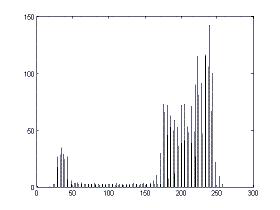
\includegraphics[scale=1]{regoines_histograma.png} 
\end{center} 

corresponde a una imagen f(x, y) compuesta por un objeto oscuro sobre un fondo claro, teniendo los p�xeles de un objeto y del entorno intensidades agrupadas en dos tonos dominantes. Una forma obvia de extraer los objetos del entorno es seleccionar un nivel T que separe los niveles de intensidad. De esta forma un p�xel (x, y) para el cual f(x, y) > T, ser� un p�xel del entorno, en caso contrario ser� del objeto.
Bas�ndonos en esto, podemos considerar la fijaci�n del umbral como una operaci�n que implica pruebas con respecto a una funci�n T como sigue:

T = T[ x, y, p(x,y), f(x,y)]

donde f(x,y) es la intensidad en el punto (x,y) y p(x,y) es alguna propiedad local del punto, por ejemplo, la intensidad media de un entorno de vecindad centrado en (x,y). Se creara una imagen binaria g(x,y) definiendo:

Si f(x,y)>T entonces g(x,y)=255 sino g(x,y)=0 fsi

Examinando g(x,y) se ve que los p�xeles a los que se asigna el valor 0 corresponden a los objetos, mientras que los que corresponden al entorno tienen valor 255.

Cuando T depende s�lo de f(x,y), el umbral se llama global. Si T depende tanto de f(x,y) como de p(x,y), entonces el umbral se llama local. Si T depende de las coordenadas espaciales x e y, se llama umbral din�mico.

\section{Extracci�n de regiones por el color}
Bas�ndonos en el modelo de color RGB, se pueden extraer de la imagen aquellas regiones en las que predomine una determinada componente de color. El m�todo consiste en elegir un determinado predicado y determinar en toda la imagen los p�xeles que cumplen dicho predicado. Esos p�xeles los marcamos en blanco y el resto en negro, de esta forma obtenemos una imagen binaria. 

\section{Selecci�n del umbral �ptimo}
Es dif�cil determinar cual es el umbral optimo para poder llevar acabo una binarizaci�n adecuada. Adem�s debemos tener en cuenta que la iluminaci�n que habr� de unas ocasiones a otras ser� distinta, esto influye en la manera en que la c�mara percibe los colores del entorno, por ejemplo, si hay poca luz los colores ser�n mas oscuros y lo contrario si hubiera mucha luz, por tanto no hemos podido determinar un umbral fijo porque este ser� dependiente del entorno.
La interfaz del pipeline genera para cada modulo de filtro una peque�a ventana que permite la elecci�n de un color de las im�genes que est�n entrando en ese momento por la webCam. De esta manera nos estamos asegurando de seleccionar y fijar el color exacto en esas condiciones del entorno. 
Debido a que las im�genes son a color, al seleccionar un color del entorno, se estar�n fijando autom�ticamente 3 umbrales, uno para el rojo, otro para el verde y otro para el azul.
Los umbrales en nuestros filtros son rangos, se podr�an considerar como un par de umbrales, uno inferior y otro superior, de tal manera que un p�xel (x,y) estar� dentro del rango si:
	Para el color rojo 	T_{inf(rojo)}<f(x,y)_{rojo}<T_{sup(rojo) }
	Para el color verde	T_{inf(verde)}<f(x,y)_{verde}<T_{sup(verde)}
	Para el color azul	T_{inf(azul)}<f(x,y) _{azul} <T_{sup(azul)}
Si las tres componentes del p�xel (x,y) est�n dentro del rango seleccionado, entonces las 3 componentes tomaran el valor blanco (255) y si estan fuera de rango tomaran el valor negro (0). Binarizando as� la imagen.

Como elegir la tolerancia de este rango. Cuanto mas amplio sea el rango mas cantidad de colores entraran dentro de este. Aunque elijamos el color exacto del entorno que queramos filtrar, si no fijamos bien la tolerancia del rango, la imagen no binarizar� las regiones correctas.

\begin{center}

\includegraphics[scale=1]{regiones_tol_baja.png} 
Extracci�n de una regi�n de color de una imagen con tolerancia baja.

\includegraphics[scale=1]{regiones_tol_normal.png} 
Extracci�n de una regi�n de color de una imagen con tolerancia normal.

\includegraphics[scale=1]{regiones_tol_alta.png} 
Extracci�n de una regi�n de color de una imagen con tolerancia alta.
\end{center} 

Para ello la ventana proporcionada por el pipeline para el filtro, no solo permite seleccionar un color determinado de la escena, sino tambi�n elegir en tiempo de ejecuci�n la tolerancia para cada rango (rojo, verde y azul). As� cada vez que el robot cambie de ambiente se puede cambiar desde su interfaz los par�metros de los 6 umbrales. As� quedar�a el color de la regi�n a extraer totalmente acotado y determinado.

Si ( T_{inf(rojo)}<f(x,y)_{rojo}<T_{sup(rojo) } and  T_{inf(verde)}<f(x,y)_{verde}<T_{sup(verde)}  and  
  T_{inf(azul)}<f(x,y) _{azul} <T_{sup(azul)}) entonces
	g(x,y)_{rojo} = 255; 	//Blanco
	g(x,y)_{verde}= 255;	//Blanco
	g(x,y)_{azul}= 255;	//Blanco
sino
	g(x,y)_{rojo} = 0; 	//Negro
	g(x,y)_{verde}= 0;	//Negro
	g(x,y)_{azul}= 0;		//Negro
fsi

Ejemplo de los 6 umbrales seleccionados en una de las puebas de extracci�n de regiones de color. 

T_{sup(rojo)}    = 170 	T_{inf(rojo) }   = 255
T_{sup(verde)} =  60	T_{inf(verde)} = 120
T_{sup(azul)}   =  70	T_{inf(azul) }  = 125

los resultados son estos:

\begin{center}

\includegraphics[scale=1]{regiones_fuente.png} 
Imagen original.

\includegraphics[scale=1]{regiones_destino.png} 
Imagen filtrada.
\end{center} 



\part{Anexo II \\ Interfaz del programador}
\label{anexo2}

\end{document}
